\documentclass[11pt]{article}
\newcommand{\ShortTitle}{STRONG ARTIN}
\usepackage[T1]{fontenc}
\usepackage[utf8]{inputenc}
\usepackage{mathpazo}
\usepackage[scaled=0.92]{helvet}
\usepackage{courier}
\usepackage{amsmath,amssymb,amsthm,mathtools}
\usepackage[a4paper,left=27mm,right=27mm,top=26mm,bottom=27mm,headheight=15pt]{geometry}
\usepackage{microtype}
\usepackage{graphicx}
\usepackage[dvipsnames]{xcolor}
\usepackage{booktabs,array,longtable,tabularx}
\usepackage{enumitem}
\usepackage{titlesec,fancyhdr}
\usepackage{caption}
\usepackage{hyperref}
\definecolor{Ink}{HTML}{243138}
\definecolor{Teal}{HTML}{21676B}
\definecolor{Copper}{HTML}{A45C36}
\definecolor{Soft}{HTML}{E9F0EF}
\definecolor{Gray}{HTML}{627078}
\hypersetup{colorlinks=true,linkcolor=Teal,citecolor=Teal,urlcolor=Teal,pdfauthor={Komorebi P.}}
\urlstyle{same}
\setlength{\parindent}{1.2em}
\setlength{\parskip}{0.15em}
\linespread{1.09}
\setlist{itemsep=0.22em,topsep=0.45em,leftmargin=1.55em}
\setlist[description]{style=nextline,leftmargin=0pt,labelwidth=0pt,labelsep=0pt,font=\normalfont\bfseries}
\setcounter{tocdepth}{2}
\setlength{\emergencystretch}{1.4em}
\titleformat{\section}{\Large\bfseries\color{Ink}}{\thesection}{0.7em}{}
\titleformat{\subsection}{\large\bfseries\color{Ink}}{\thesubsection}{0.7em}{}
\titleformat{\subsubsection}{\normalsize\bfseries\color{Ink}}{\thesubsubsection}{0.7em}{}
\titlespacing*{\section}{0pt}{1.8em}{0.7em}
\titlespacing*{\subsection}{0pt}{1.3em}{0.5em}
\captionsetup{font=small,labelfont={bf,color=Teal},skip=8pt}
\pagestyle{fancy}
\fancyhf{}
\fancyhead[L]{\sffamily\scriptsize\color{Gray}OPERATION KOMOREBI}
\fancyhead[R]{\sffamily\scriptsize\color{Gray}\ShortTitle}
\fancyfoot[L]{\sffamily\scriptsize\color{Gray}CONJECTURE SERIES / 8 OCTOBER 2026}
\fancyfoot[R]{\sffamily\small\color{Ink}\thepage}
\renewcommand{\headrulewidth}{0.25pt}
\renewcommand{\footrulewidth}{0pt}
\theoremstyle{plain}
\newtheorem{theorem}{Theorem}[section]
\newtheorem{proposition}[theorem]{Proposition}
\newtheorem{lemma}[theorem]{Lemma}
\newtheorem{corollary}[theorem]{Corollary}
\newtheorem{conjecture}[theorem]{Conjecture}
\theoremstyle{definition}
\newtheorem{definition}[theorem]{Definition}
\newtheorem{example}[theorem]{Example}
\theoremstyle{remark}
\newtheorem{remark}[theorem]{Remark}
\newtheorem{hypothesis}[theorem]{Hypothesis}
\numberwithin{equation}{section}
\providecommand{\N}{\mathbb N}
\providecommand{\Z}{\mathbb Z}
\providecommand{\Q}{\mathbb Q}
\providecommand{\R}{\mathbb R}
\providecommand{\C}{\mathbb C}
\providecommand{\eps}{\varepsilon}
\providecommand{\dd}{\mathrm d}
\providecommand{\norm}[1]{\left\lVert #1\right\rVert}
\providecommand{\abs}[1]{\left\lvert #1\right\rvert}
\graphicspath{{../shared/figures/}}
\newcommand{\figplaceholder}[2]{\begin{figure}[tbp]\centering\includegraphics[width=0.97\linewidth]{#1.pdf}\caption{#2}\label{fig:#1}\end{figure}}
\newcommand{\Cover}[4]{%
\hypersetup{pageanchor=false}
\begin{titlepage}\thispagestyle{empty}
\noindent{\sffamily\small\color{Teal}OPERATION KOMOREBI\hfill CONJECTURE SERIES #1}\par
\vspace{27mm}
\noindent{\fontsize{43}{47}\selectfont\color{Ink}#2}\par
\vspace{5mm}\noindent{\LARGE\color{Ink}#3}\par
\vspace{9mm}\noindent{\color{Teal}\rule{\linewidth}{1.1pt}}\par
\vspace{8mm}\noindent{\large Komorebi P.}\par
\vspace{2mm}\noindent{\sffamily\small\color{Gray}READER EDITION 1.0 / 8 OCTOBER 2026}\par
\vfill
\noindent\begin{minipage}{0.96\linewidth}{\large\color{Ink}#4}\end{minipage}\par
\vspace{9mm}\noindent{\sffamily\small\color{Teal}EXACT IDENTITIES\quad /\quad FINITE EVIDENCE\quad /\quad OPEN CONJECTURE}\par
\end{titlepage}\hypersetup{pageanchor=true}}

\usepackage[nameinlink,noabbrev]{cleveref}
\allowdisplaybreaks
\newtheorem{standardfact}[theorem]{Classical input}
\crefname{standardfact}{classical input}{classical inputs}
\crefname{hypothesis}{hypothesis}{hypotheses}
\newcommand{\CC}{\mathbb C}
\newcommand{\QQ}{\mathbb Q}
\newcommand{\ZZ}{\mathbb Z}
\newcommand{\FF}{\mathbb F}
\newcommand{\Adele}{\mathbb A}
\newcommand{\GL}{\operatorname{GL}}
\newcommand{\Gal}{\operatorname{Gal}}
\newcommand{\Frob}{\operatorname{Frob}}
\newcommand{\Tr}{\operatorname{Tr}}
\newcommand{\Hom}{\operatorname{Hom}}
\newcommand{\Ind}{\operatorname{Ind}}
\newcommand{\Res}{\operatorname{Res}}
\newcommand{\Irr}{\operatorname{Irr}}
\newcommand{\rec}{\operatorname{rec}}
\newcommand{\BC}{\operatorname{BC}}
\newcommand{\AI}{\operatorname{AI}}
\newcommand{\ord}{\operatorname{ord}}
\newcommand{\Supp}{\operatorname{Supp}}
\newcommand{\im}{\operatorname{im}}
\newcommand{\calJ}{\mathcal J}
\newcommand{\calX}{\mathcal X}
\newcommand{\calE}{\mathcal E}
\newcommand{\calC}{\mathcal C}
\newcommand{\calP}{\mathcal P}
\newcommand{\calQ}{\mathcal Q}
\newcommand{\muP}{\boldsymbol\mu_p}
\newcommand{\OO}{\mathcal O}
\newcommand{\frakl}{\mathfrak l}
\newcommand{\calA}{\mathcal A}
\newcommand{\calB}{\mathcal B}
\newcommand{\calF}{\mathcal F}
\newcommand{\one}{\mathbf 1}
\graphicspath{{../visual/figures/}}
\hypersetup{pdftitle={Strong Artin: Cyclic Attachment, Finite Alphabets, and the Global Realization Gap},pdfsubject={Conjecture series, finite representation proofs, residual realization, and certified local lifting}}
\begin{document}
\Cover{03}{Strong Artin}{Cyclic attachment and finite realization}{A detailed account of the representation theory, exact selectors, realization criteria, and certified local lifting sectors. The global automorphic attachment remains open.}
\tableofcontents
\newpage
\section{The conjecture and the work represented here}\label{sec:introduction}

A finite Galois representation presents a strikingly discrete object. Its matrices range over a finite group. At an unramified prime, its Frobenius eigenvalues are roots of unity. The Strong Artin conjecture asks that this discrete arithmetic information occur inside the automorphic spectrum, with the correct dimension, local parameters, and global analytic structure. Knowing a finite list of possible eigenvalues does not supply the automorphic representation that should carry them.

This piece studies that distinction at a cyclic descent step. There are exact finite choices on both sides of the proposed correspondence. The choices can be described, separated, and tested. What remains is a theorem that identifies a choice on the automorphic side with the prescribed arithmetic object. Later local deformation and matrix lifting results sharpen several algebraic parts of that problem. They do not manufacture the global automorphic carrier.

\subsection{Two strengths of attachment}

Let \(F\) be a number field, let \(G_F=\Gal(\overline F/F)\), and let
\[
 \rho:G_F\longrightarrow\GL_n(\CC)
\]
be a continuous representation with finite image. Continuity is taken for the usual complex topology. Such a representation factors through the Galois group of a finite extension. Throughout the conjecture discussion, \(\rho\) is irreducible. The trivial one dimensional representation is excluded when discussing entireness of an Artin \(L\) function, since its \(L\) function is the Dedekind zeta function.

At a finite place where \(\rho\) is unramified, fix the Frobenius convention used by the normalized local Langlands correspondence. Write
\[
 P_{\rho,v}(T)=\det\bigl(TI_n-\rho(\Frob_v)\bigr).
\]
For an unramified automorphic local component \(\pi_v\), write \(P_{\pi,v}(T)\) for the monic polynomial of its normalized Satake conjugacy class. The convention is chosen so that an attached pair has the same polynomial. This keeps a possible geometric versus arithmetic Frobenius inversion from entering a comparison silently.

\begin{conjecture}[Strong Artin, unramified form]\label{conj:strong_artin_weak}
Every irreducible finite image complex representation \(\rho\) of \(G_F\) has a cuspidal automorphic representation \(\pi\) of \(\GL_n(\Adele_F)\) such that
\[
 P_{\pi,v}(T)=P_{\rho,v}(T)
\]
for all finite places outside a finite set.
\end{conjecture}

We call this weak attachment, where weak refers to the comparison at almost all unramified places. It remains a powerful global assertion. It implies the expected unramified Euler factors and identifies the cuspidal automorphic representation uniquely by strong multiplicity one.

\begin{conjecture}[Strong Artin, all local form]\label{conj:strong_artin_full}
The representation \(\pi\) can be chosen so that
\[
 \rec_{F_v}(\pi_v)\cong\rho|_{W_{F_v}}
\]
for every place \(v\), with zero monodromy at finite places.
\end{conjecture}

At a finite place, the right side is viewed as a Weil Deligne representation with monodromy operator zero. At an archimedean place, the statement uses the corresponding archimedean parameter. The all local assertion includes ramified and infinity data that do not appear in the definition of weak attachment. In this piece an unramified comparison is never silently promoted to an all local theorem. A residual realization will first give weak attachment. The remaining finite set of local parameters must then be checked or covered by an additional compatibility theorem.

\subsection{The classical range and the new boundary}

Class field theory handles dimension one. Cyclic base change and automorphic induction provide powerful higher dimensional constructions. An induction step is available when its field tower and cuspidality conditions fall within the established induction formalism. We do not assert that every abstract monomial character has an automorphic realization merely because it is induced from a linear character. The relevant field and induction chain must be covered by a theorem \cite{ArthurClozel1989}.

The solvable two dimensional sectors treated by Langlands and Tunnell, further examples such as the solvable \(\mathrm{GO}(4)\) range, and other established cases show that the conjecture is far from an empty expectation \cite{Langlands1980,Tunnell1981,Ramakrishnan2002}. A recent preprint of Wang states the generalized octahedral \(\GL_3\) case with projective image \(C_3^2\rtimes\mathrm{SL}(2,3)\), together with a primitive solvable six dimensional consequence \cite{Wang2026}. Its stated results have been checked against the submitted source. Its full proof has not been independently audited for this edition. These particular sectors must therefore not be described as untouched simply because the general problem remains open.

Arthur and Clozel's prime degree cyclic constructions and the descent and fibre statements clarified by Clozel and Rajan are the external automorphic inputs used below \cite{ArthurClozel1989,ClozelRajan2020}. For a cyclic extension, an invariant unitary cuspidal representation descends. When its base change is cuspidal, the cuspidal descents differ by quotient characters, and these twists are distinct. The more general solvable base change statement has extra twisting information. We use the precise prime cyclic case in the recursive argument.

The finite representation arguments have a parallel shape. If \(H\triangleleft G\) and \(G/H\cong C_p\), an irreducible representation either restricts to a full orbit of \(p\) subgroup types or restricts irreducibly to one invariant type. In the first case induction reconstructs the representation. In the second case an extension must be selected. The second case is where two torsors meet. Each torsor exists, and each has \(p\) elements. There is no preferred origin in the statement that they are torsors under the same character group.

\subsection{What the finite analysis proves}

The core argument retains the detailed residual realization analysis of the earlier project source. Stable subgroup types carry multiplicity spaces on which the cyclic quotient acts. Their ordered character multiplicities are recorded in polynomials
\[
 P_{\tau,V}(z)=\sum_{a\in\ZZ/p\ZZ}m_{\tau,a}(V)z^a.
\]
A quotient twist rotates every such polynomial by the same amount. Moving subgroup types carry induced blocks and do not retain a quotient label. This gives a complete extension comparison, not just a determinant or total trace test.

At each place, a finite alignment set records the quotient labels that attach the local automorphic parameter to the target. The all local cyclic step is equivalent to a common label in all these sets. A nonempty exact alignment set is a coset of a subgroup of \(C_p\), so it is a singleton or the whole label group. It may also be empty. The reduction makes the missing statement precise. It does not show that the local requirements are compatible.

A second chain starts with a descent whose base change is already of Artin type. Every descended local parameter has finite image. Every unramified Satake root belongs to one finite cyclotomic group. Consequently the Hecke polynomial alphabet is finite, its coefficients are integral, and all but finitely many coefficient primes separate its entries. A finite trace argument then bounds a semisimple residual image. A sufficiently large residual realization lifts in cross characteristic and is forced onto the exact characteristic zero polynomial alphabet. At a good separating prime, even the smaller direct torsor argument recovers the cyclic offset.

The same trace pairing gives an especially direct proof for an ordinary semisimple \(\ell\) adic realization. Chebotarev and continuity extend a finite Frobenius trace alphabet to every image element. The semisimple image algebra then embeds the image in a finite Cartesian power of that alphabet. Thus the image is finite. The existence of the \(\ell\) adic representation remains the input. The finite image conclusion is the output.

A third phenomenon occurs at the quotient prime \(p\). The order \(p\) characters all reduce to the trivial character, and the unramified cyclic base change identities force the automorphic and target polynomial systems to agree modulo a coefficient prime above \(p\). This congruence cannot choose a characteristic zero label. It is the beginning of a lifting problem. It supplies neither a residual Galois representation for an arbitrary automorphic descent nor an unrestricted automorphy lifting theorem for repeated weight zero parameters.

\subsection{How to read the formal and computational record}

The second part develops the later local results. Cyclic first cohomology describes infinitesimal conjugacy ambiguity under its stated norm condition. Second cohomology records a square zero extension defect. Syzygy calculations identify redundant local prescriptions after an explicit arithmetic comparison is supplied. Ordered matrix Hensel lifting gives an actual root from one finite congruence when a two sided inverse derivative certificate is available and the prescribed ball is sufficiently small. The noncommutative order of the derivative is part of the theorem.

These are useful closed sectors. They are not a proof that every arithmetic local obstruction vanishes, that every simultaneous prescription is realizable, or that a global automorphic carrier exists. The distinction is carried through the hypotheses, examples, and final statement map. A noncommuting positive matrix control and a rejected target show the local criterion working in both directions. A genuinely singular derivative exhibits the sector outside that criterion.

The accompanying sources retain historical verification reports and the precise formal statement boundaries. A historical Lean certificate verifies the theorem encoded in its source under its hypotheses. It does not verify an unstated arithmetic identification or fill a missing global premise. New computations in this edition are bounded checks of exact finite identities and figures. Their ranges are documented, and their counts are not added to overlapping historical suites as though every check were independent.

No unrestricted Strong Artin theorem and no global novelty claim is made here. The point is a substantial, inspectable body of mathematics around the remaining gate: exact representation theory, finite selectors, rigidity, local lifting, and a clear statement of what a successful global realization theorem would still have to provide.

\section{Cyclic extension and descent torsors}\label{sec:torsors}

Let \(G\) be a finite group, let \(H\triangleleft G\), and assume
\[
 G/H\cong C_p
\]
for a prime \(p\). Let \(X=\Hom(G/H,\CC^\times)\), which is cyclic of order \(p\).

\begin{proposition}[Galois extension torsor]\label{prop:galois_torsor}
Let \(\tau\) be an irreducible complex representation of \(H\) that is invariant under \(G\), and suppose \(\tau\) extends to an irreducible representation of \(G\). Then the set of isomorphism classes of extensions of \(\tau\) to \(G\) is an \(X\) torsor under tensor product.
\end{proposition}

\begin{proof}
Fix one extension \(\rho\). Every \(\chi\in X\) is trivial on \(H\), so \(\rho\otimes\chi\) restricts to \(\tau\). Conversely, let \(\rho'\) be another extension. Since both restrictions are irreducible and isomorphic, Schur's lemma shows that after one choice of an \(H\) intertwiner, the ratio between the two actions is scalar on each coset. Those scalars define a character of \(G/H\), so \(\rho'\cong\rho\otimes\chi\).

The action is free. If \(\rho\cong\rho\otimes\chi\), an intertwiner restricts to a scalar on \(H\). Commuting it through one element outside \(H\) gives \(\chi=1\).
\end{proof}

\begin{standardfact}[Prime cyclic cuspidal descent and fibre]\label{fact:base_change_fibre}
Let \(E/F\) be cyclic of prime degree, and let \(\Pi\) be an invariant unitary cuspidal representation of \(\GL_n(\Adele_E)\). Then \(\Pi\) has a cuspidal descent to \(F\). Its cuspidal descents form a torsor under the Hecke characters corresponding by class field theory to \(\Gal(E/F)\). In particular, distinct quotient twists of one descent remain distinct. We use the prime cyclic construction of Arthur and Clozel and the fibre statement and cyclic descent clarification of Clozel and Rajan \cite{ArthurClozel1989,ClozelRajan2020}. The assertion concerns a cuspidal base change. It is not a claim that quotient twisting acts freely on every cuspidal representation.
\end{standardfact}

\begin{definition}[Attached cyclic descent]\label{def:attached_descent}
Let \(E/F\) be cyclic of prime degree \(p\), and let \(\rho\) be an irreducible finite image representation of \(G_F\) whose restriction \(\tau=\rho|_{G_E}\) is irreducible. Suppose \(\tau\) is automorphic with cuspidal representation \(\Pi\) of \(\GL_n(\Adele_E)\). An attached cyclic descent is a cuspidal descent \(\pi\) of \(\Pi\) such that
\[
 \rec_{F_v}(\pi_v)
 \cong
 \rho|_{W_{F_v}}
\]
for every place \(v\) of \(F\).
\end{definition}

\begin{proposition}[One attachment determines the whole fibre]\label{prop:one_attachment}
If one attached cyclic descent exists, then every Galois extension in the torsor of \cref{prop:galois_torsor} is attached to the corresponding quotient twist of that descent.
\end{proposition}

\begin{proof}
Local class field theory identifies a quotient character \(\chi\in X\) with the corresponding Hecke character. Local Langlands is compatible with character twisting, \cite{HarrisTaylor2001}. Hence
\[
 \rec(\pi_v\otimes\chi_v)
 \cong
 \rec(\pi_v)\otimes\chi_v
 \cong
 \rho_v\otimes\chi_v.
\]
The result holds at every place.
\end{proof}

\begin{corollary}[Clifford recursion reduction]\label{cor:clifford_reduction}
Suppose a finite solvable image representation is followed down a prime cyclic Clifford tower. Every induction step is handled by automorphic induction. If attached cyclic descent holds at every invariant extension step, then the original representation satisfies Strong Artin.
\end{corollary}

\begin{proof}
Start at a one dimensional bottom constituent, which is automorphic by class field theory. Move upward through the tower. Use automorphic induction at each induction step and attached cyclic descent at each invariant extension step. The local parameters remain those of the Galois representation at every stage.
\end{proof}

\begin{figure}[tbp]\centering
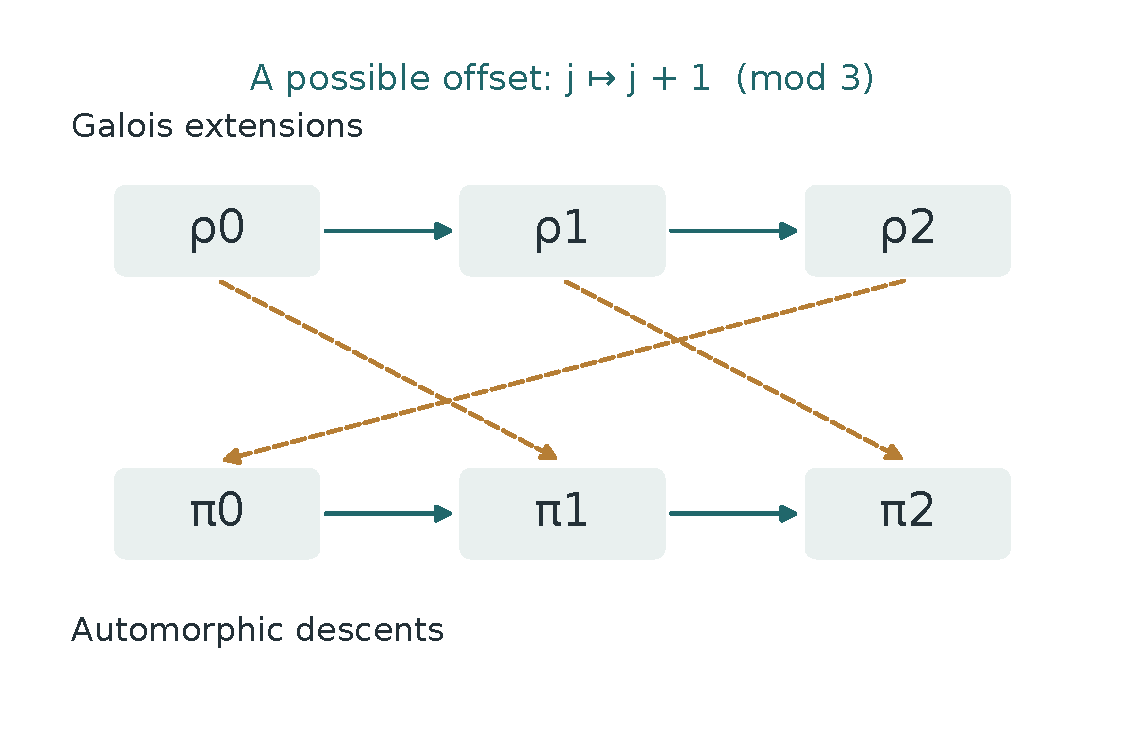
\includegraphics[width=.88\linewidth]{03_torsor.pdf}
\caption{A quotient character rotates the two cyclic torsors. Neither torsor has a preferred origin, so the common character action does not specify their attachment.}
\label{fig:cyclic_torsors}\end{figure}

\section{Coefficient selectors in a cyclic fibre}\label{sec:selectors}

Let \(\xi\) be a generator of \(X\), and identify its values with \(p\)th roots of unity. For a matrix \(A\in\GL_n(\CC)\), write
\[
 \det(TI-A)
 =
 \sum_{k=0}^{n}(-1)^k e_k(A)T^{n-k}.
\]

\begin{proposition}[Coefficient rotation]\label{prop:coefficient_rotation}
For \(\zeta\in\CC^\times\),
\[
 \boxed{
 e_k(\zeta A)=\zeta^k e_k(A).
 }
\]
\end{proposition}

\begin{proof}
The coefficient \(e_k(A)\) is the trace of \(\bigwedge^k A\). Scalar multiplication by \(\zeta\) acts on \(\bigwedge^k\CC^n\) by \(\zeta^k\).
\end{proof}

\begin{definition}[Active coefficient degrees]\label{def:active_degrees}
Define
\[
 S(A)=\{k\in\{1,\ldots,n\}:e_k(A)\neq0\}.
\]
\end{definition}

\begin{theorem}[One polynomial separator]\label{thm:one_polynomial_separator}
Let \(\zeta\) range over \(\mu_p\). The twists \(\zeta A\) have pairwise distinct characteristic polynomials exactly when \(S(A)\) contains a degree not divisible by \(p\).
\end{theorem}

\begin{proof}
By \cref{prop:coefficient_rotation}, the stabilizer of the characteristic polynomial is
\[
 \{\zeta\in\mu_p:\zeta^k=1\text{ for every }k\in S(A)\}.
\]
Since \(p\) is prime, a nontrivial \(p\)th root satisfies \(\zeta^k=1\) exactly when \(p\mid k\).
\end{proof}

\begin{corollary}[Trace and determinant selectors]\label{cor:trace_det_selector}
A nonzero trace separates all cyclic twists. The determinant separates all cyclic twists when \(p\nmid n\).
\end{corollary}

\begin{proof}
Use degree one for the trace and degree \(n\) for the determinant in \cref{thm:one_polynomial_separator}.
\end{proof}

\begin{theorem}[Determinant selector for extension torsors]\label{thm:determinant_selector}
Assume \(p\nmid n\). In the Galois extension torsor of an \(n\) dimensional irreducible representation, the determinant distinguishes all \(p\) extensions. In the automorphic descent torsor, the central character distinguishes all \(p\) descents. Both transformations are equivariant under the \(n\)th power map on \(X\).
\end{theorem}

\begin{proof}
For a quotient character \(\chi\),
\[
 \det(\rho\otimes\chi)=\det(\rho)\chi^n.
\]
The central character satisfies the identical formula
\[
 \omega_{\pi\otimes\chi}=\omega_\pi\chi^n.
\]
Since \(X\) has prime order \(p\) and \(p\nmid n\), the map \(\chi\mapsto\chi^n\) is an automorphism of \(X\).
\end{proof}

\begin{theorem}[Unique determinant matched descent]\label{thm:determinant_matched_descent}
Use the cyclic Artin setup of \cref{def:attached_descent}, and assume \(p\nmid n\). Let \(\pi_0\) be any cuspidal descent of \(\Pi\). Then there is a unique quotient character \(\chi\in X\) such that
\[
 \boxed{
 \omega_{\pi_0\otimes\chi}
 =
 \det\rho
 }
\]
under global class field theory.
\end{theorem}

\begin{proof}
The base change of \(\omega_{\pi_0}\) is the central character of \(\Pi\). Since \(\Pi\) is attached to \(\tau=\rho|_{G_E}\), that character equals \(\det\tau\). The base change of \(\det\rho\) is also \(\det\tau\). Hence
\[
 \delta=(\det\rho)\omega_{\pi_0}^{-1}
\]
is a character killed by base change to \(E\), so \(\delta\in X\). We need \(\chi^n=\delta\). Since \(X\) has order \(p\) and \(p\nmid n\), the \(n\)th power map on \(X\) is bijective. Thus there is one and only one such \(\chi\).
\end{proof}

\begin{corollary}[Rank prime sieve]\label{cor:rank_prime_sieve}
At a cyclic prime step of degree \(p\), determinant data leaves no torsor ambiguity unless \(p\mid n\). The only quotient primes invisible to determinant selection are prime divisors of the rank.
\end{corollary}

\begin{proof}
This is \cref{thm:determinant_selector}.
\end{proof}

\begin{remark}\label{rem:determinant_not_attachment}
Matching determinant and central character selects a unique candidate descent when \(p\nmid n\). It does not prove that the remaining local characteristic polynomials match. The selection theorem removes the finite torsor ambiguity, not the global realization problem.
\end{remark}

\section{Two no go theorems for invisible cyclic twists}\label{sec:no_go}

The determinant selector is optimal among algebraic central characters. When the quotient prime divides the rank, applying more algebraic functors does not repair it.

\begin{proposition}[Determinant character of an algebraic representation]\label{prop:algebraic_det_character}
Let
\[
 r:\GL_n(\CC)\longrightarrow\GL_N(\CC)
\]
be an irreducible algebraic representation. Suppose the center acts with weight \(w\), so
\[
 r(zI_n)=z^wI_N.
\]
There is an integer \(a\) such that
\[
\boxed{
 \det r(g)=\det(g)^a
}
\]
and
\[
\boxed{
 wN=an.
}
\]
\end{proposition}

\begin{proof}
Every algebraic character of \(\GL_n\) is an integral power of the determinant. Thus \(\det\circ r=\det^a\) for one integer \(a\). Evaluate both sides at \(zI_n\). The left side is \(z^{wN}\), while the right side is \(z^{an}\).
\end{proof}

\begin{theorem}[Algebraic central characters are blind when \(p\mid n\)]\label{thm:central_character_no_go}
Let \(\chi\) have order \(p\), and assume \(p\mid n\). For every irreducible algebraic representation \(r\) of \(\GL_n\),
\[
\boxed{
 \det r(\rho\otimes\chi)=\det r(\rho).
}
\]
The same statement holds on every irreducible summand of an arbitrary finite dimensional algebraic representation.
\end{theorem}

\begin{proof}
The scalar twist acts on \(r(\rho)\) by \(\chi^w\). Hence its determinant changes by \(\chi^{wN}\). By \cref{prop:algebraic_det_character}, \(wN=an\), which is divisible by \(p\). Thus \(\chi^{wN}=1\). Apply the argument to each irreducible summand.
\end{proof}

\begin{corollary}[Optimality of the rank prime sieve]\label{cor:rank_sieve_optimal}
When \(p\mid n\), no finite collection of determinant or central character tests obtained from algebraic functors on \(\GL_n\) can distinguish the order \(p\) scalar extension twists.
\end{corollary}

\begin{proof}
Every test in the collection is invariant by \cref{thm:central_character_no_go}.
\end{proof}

\begin{standardfact}[Stable equality of epsilon factors]\label{fact:epsilon_stability}
Let \(V,V'\) be finite dimensional complex Weil representations with finite inertia image, of equal dimension and determinant. For every sufficiently ramified auxiliary character \(\eta\),
\[
 \epsilon(V\otimes\eta,\Psi)=\epsilon(V'\otimes\eta,\Psi).
\]
Here \(\Psi\) is a fixed nontrivial additive character and the same normalization is used on both sides. Deligne and Henniart's stability theorem applies to the virtual representation \(B=V-V'\), which has dimension zero and determinant one. Their Theorem 4.6 gives the ratio as a determinant evaluation once the slope of \(\eta\) exceeds twice the largest relevant slope of \(B\). That ratio is one \cite{DeligneHenniart1981}. We use this equality and avoid an unspecified choice of the auxiliary determinant evaluation element.
\end{standardfact}

\begin{theorem}[Highly ramified epsilon twists are blind]\label{thm:epsilon_no_go}
Let \(V' = V\otimes\chi\), where \(\chi\) has order \(p\), and assume \(p\mid\dim V\). Then \(V\) and \(V'\) have the same determinant. For every sufficiently ramified auxiliary character \(\eta\),
\[
\boxed{
 \epsilon(V\otimes\eta,\Psi)
 =
 \epsilon(V'\otimes\eta,\Psi).
}
\]
\end{theorem}

\begin{proof}
The determinant changes by \(\chi^{\dim V}=1\). The two representations have the same dimension and determinant. Apply \cref{fact:epsilon_stability}.
\end{proof}

\begin{remark}\label{rem:no_go_boundary}
When the quotient prime divides the rank, neither algebraic central characters nor sufficiently ramified epsilon twists see the cyclic label. Any complete attachment theorem must use bounded depth noncentral local data, a genuine Galois realization, or an automorphy lifting theorem that controls the corresponding local component.
\end{remark}

\begin{theorem}[The total induced object is torsor blind]\label{thm:total_induction_blind}
Let \(H\triangleleft G\) with cyclic quotient character group \(X\), and let \(V\) be an extension of an \(H\) representation. Then
\[
\boxed{
 \bigoplus_{\chi\in X}
 V\otimes\chi
 \cong
 \Ind_H^G\Res_HV.
}
\]
The left side is unchanged when \(V\) is replaced by another member of its extension torsor. Likewise, for cyclic base change,
\[
\boxed{
 \mathop{\boxplus}_{\chi\in X}
 \pi\otimes\chi
 \cong
 \AI_{E/F}(\BC_{E/F}\pi)
}
\]
inside the established automorphic induction formalism. Therefore comparison of the total induced objects cannot determine the cyclic attachment offset.
\end{theorem}

\begin{proof}
The restriction of every quotient character to \(H\) is trivial. The regular representation of \(G/H\) decomposes as the direct sum of all characters in \(X\). Hence
\[
 \Ind_H^G\Res_HV
 \cong
 V\otimes\CC[G/H]
 \cong
 \bigoplus_{\chi\in X}V\otimes\chi.
\]
Replacing \(V\) by \(V\otimes\chi_0\) only permutes the summands. The automorphic identity is the cyclic automorphic induction and base change analogue. It has the same permutation invariance.
\end{proof}

\begin{figure}[tbp]\centering
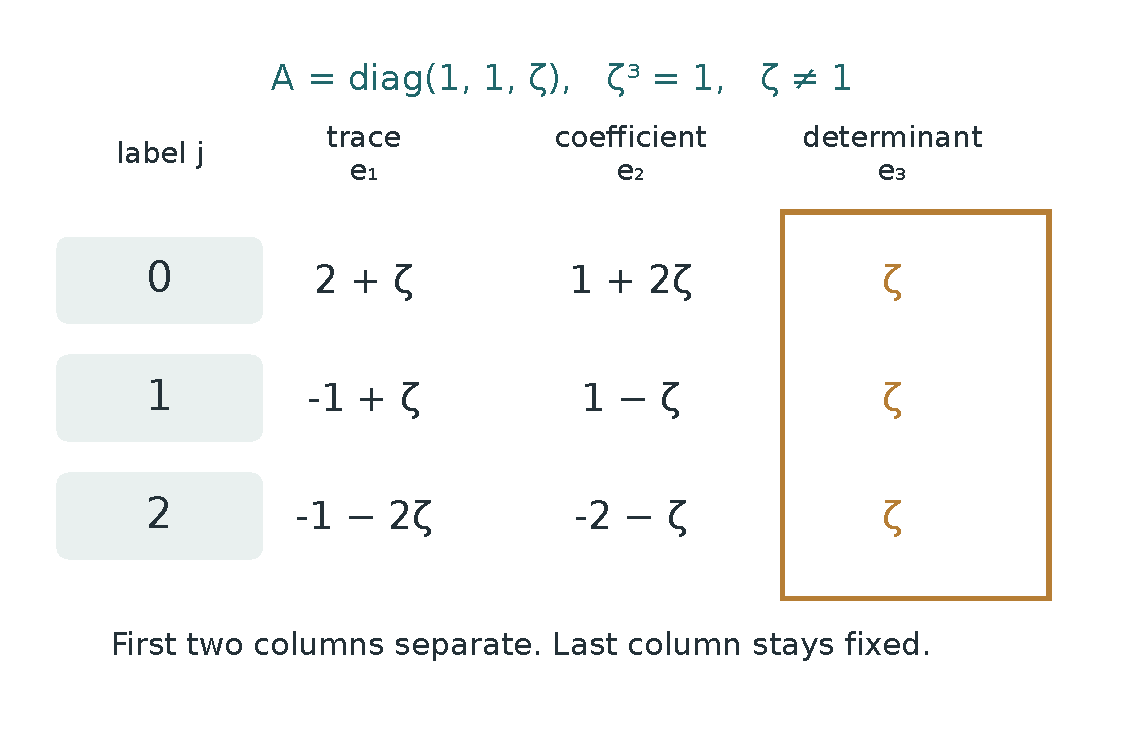
\includegraphics[width=.90\linewidth]{08_blindness.pdf}
\caption{At quotient prime three and rank three, determinant is fixed by the scalar twist. Lower coefficient degrees can still detect the label when their coefficients are nonzero.}
\label{fig:determinant_blindness}\end{figure}

\section{Local extension spectra}\label{sec:extension_spectra}

The determinant is only one aggregate of the local cyclic extension labels. Clifford theory gives the complete finite invariant.

Let \(G/H\cong C_p\), and choose a quotient character \(\xi\). Let \(G\) be finite and let \(V\) be a finite dimensional semisimple complex representation of \(G\).

\begin{definition}[Stable and moving types]\label{def:stable_moving}
An irreducible representation \(\tau\in\Irr(H)\) is stable when \(\tau^g\cong\tau\) for every \(g\in G\). Otherwise its orbit has size \(p\) and is called moving.
\end{definition}

\begin{lemma}[Extension of a stable type]\label{lem:stable_extension}
Every stable irreducible complex representation of \(H\) extends to \(G\).
\end{lemma}

\begin{proof}
Choose \(g\in G\) whose class generates \(G/H\), so \(g^p\in H\). Stability gives an invertible intertwiner \(A\) with
\[
 A\tau(h)A^{-1}=\tau(ghg^{-1})\qquad(h\in H).
\]
Iterate this identity \(p\) times. The operator \(\tau(g^p)^{-1}A^p\) commutes with \(\tau(H)\), so Schur's lemma makes it a nonzero scalar \(cI\). Also \(A\) commutes with \(\tau(g^p)\), by the same intertwining identity at \(h=g^p\). Choose \(b\in\CC^\times\) with \(b^p=c^{-1}\) and put \(R=bA\). Then
\[
 R\tau(h)R^{-1}=\tau(ghg^{-1}),\qquad R^p=\tau(g^p).
\]
These are exactly the conjugation and closing relations for the coset presentation of \(G\). Assigning \(g\mapsto R\) and \(h\mapsto\tau(h)\) therefore defines a representation of \(G\) extending \(\tau\). Its restriction is irreducible, so the extension is irreducible. In cohomological language the scalar cyclic obstruction vanishes because a nonzero complex number has a \(p\)th root. This uses the coefficient field, and must not be transplanted unchanged into an arbitrary integral or residual lifting problem.
\end{proof}

Fix one extension \(\widetilde\tau\) for every stable \(\tau\).

\begin{definition}[Extension spectrum polynomial]\label{def:extension_spectrum}
For a stable type \(\tau\), the multiplicity space
\[
 M_\tau(V)=\Hom_H(\tau,V)
\]
becomes a representation of \(G/H\) after comparing the action on \(V\) with \(\widetilde\tau\). Write
\[
 M_\tau(V)
 \cong
 \bigoplus_{a\in\ZZ/p\ZZ}
 (\xi^a)^{\oplus m_{\tau,a}(V)}.
\]
Define
\[
 \boxed{
 P_{\tau,V}(z)
 =
 \sum_{a\in\ZZ/p\ZZ}
 m_{\tau,a}(V)z^a
 }
\]
in \(\ZZ[z]/(z^p-1)\).
\end{definition}

\begin{proposition}[Effect of quotient twisting]\label{prop:spectrum_twist}
For every \(j\in\ZZ/p\ZZ\),
\[
 \boxed{
 P_{\tau,V\otimes\xi^j}(z)
 =
 z^jP_{\tau,V}(z).
 }
\]
Moving orbit blocks are unchanged up to isomorphism by quotient twisting.
\end{proposition}

\begin{proof}
The quotient character acts only on the multiplicity space, shifting every character label by \(j\). For a moving type, its inertia group is \(H\), and the corresponding irreducible block is induced from \(H\). Tensoring an induced representation by a character trivial on \(H\) produces an isomorphic induced representation.
\end{proof}

\begin{theorem}[Cyclic extension spectrum criterion]\label{thm:extension_spectrum_criterion}
Let \(V\) and \(W\) be semisimple representations of \(G\) with
\[
 \Res_HV\cong\Res_HW.
\]
Then
\[
 \boxed{
 W\cong V\otimes\xi^j
 }
\]
for some \(j\in\ZZ/p\ZZ\) if and only if, for every stable irreducible \(H\) type \(\tau\),
\[
 \boxed{
 P_{\tau,W}(z)
 =
 z^jP_{\tau,V}(z).
 }
\]
The moving orbit blocks require no additional condition.
\end{theorem}

\begin{proof}
Decompose the restriction to \(H\) into \(G\) orbits of irreducible types. For a moving orbit, Clifford theory gives one irreducible induced block, with multiplicity determined by the restriction. Quotient twisting fixes its isomorphism class.

For a stable type \(\tau\), the full \(\tau\) isotypic contribution is
\[
 \widetilde\tau\otimes M_\tau(V).
\]
The corresponding contribution for \(W\) is determined by \(M_\tau(W)\). Tensoring by \(\xi^j\) shifts every quotient character in every stable multiplicity space by the same \(j\). Thus the displayed polynomial identities are necessary and sufficient on each stable block. Direct sum over all blocks gives the result.
\end{proof}

\begin{definition}[Alignment set]\label{def:alignment_set}
For \(V,W\) with the same restriction to \(H\), define
\[
 \boxed{
 \calJ_H(V,W)
 =
 \{j\in\ZZ/p\ZZ:
 P_{\tau,W}=z^jP_{\tau,V}
 \text{ for every stable }\tau\}.
 }
\]
\end{definition}

\begin{corollary}[Structure of the alignment set]\label{cor:alignment_coset}
The alignment set is empty or a coset of the common rotational stabilizer
\[
 \bigcap_\tau
 \{j:z^jP_{\tau,V}=P_{\tau,V}\}.
\]
In particular, one stable type with aperiodic spectrum makes the alignment index unique whenever it exists.
\end{corollary}

\begin{proof}
If \(j_0\) is one solution, every other solution differs from it by a rotation stabilizing every spectrum polynomial. The converse is immediate.
\end{proof}

\begin{example}[Irreducible stable restriction]\label{ex:irreducible_stable}
If \(\Res_HV\) is irreducible, its multiplicity polynomial is one monomial. Hence \(\calJ_H(V,W)\) is a singleton. This recovers the ordinary extension torsor of \cref{prop:galois_torsor}.
\end{example}



\subsection{Fourier coordinates of an extension spectrum}

Fix a primitive \(p\)th root \(\zeta\). For
\[
 P(z)=\sum_{a\in\ZZ/p\ZZ}m_az^a,
\]
define
\[
 \widehat P(r)
 =
 \sum_{a\in\ZZ/p\ZZ}m_a\zeta^{ar},
 \qquad
 r\in\ZZ/p\ZZ.
\]

\begin{proposition}[Fourier trace interpretation]\label{prop:fourier_trace}
Let \(g\) be a lift of a generator of \(G/H\). For a stable type \(\tau\),
\[
 \boxed{
 \widehat P_{\tau,V}(r)
 =
 \Tr\left(g^r\mid M_\tau(V)\right).
 }
\]
If \(V\) is twisted by \(\xi^j\), then
\[
 \boxed{
 \widehat P_{\tau,V\otimes\xi^j}(r)
 =
 \zeta^{jr}\widehat P_{\tau,V}(r).
 }
\]
\end{proposition}

\begin{proof}
The quotient generator acts on the \(\xi^a\) summand by \(\zeta^a\). Taking the trace of its \(r\)th power gives the Fourier sum. The twist multiplies the action of \(g^r\) by \(\zeta^{jr}\).
\end{proof}

\begin{corollary}[Fourier attachment test]\label{cor:fourier_attachment}
Suppose \(\Res_HV\cong\Res_HW\). Then \(W\cong V\otimes\xi^j\) if and only if
\[
 \boxed{
 \widehat P_{\tau,W}(r)
 =
 \zeta^{jr}\widehat P_{\tau,V}(r)
 }
\]
for every stable type \(\tau\) and every \(r\in\ZZ/p\ZZ\).
\end{corollary}

\begin{proof}
The discrete Fourier transform on \(\ZZ/p\ZZ\) is invertible. Thus the Fourier identities are equivalent to the polynomial shift identities in \cref{thm:extension_spectrum_criterion}.
\end{proof}

\begin{corollary}[One nonzero Fourier mode selects the shift]\label{cor:one_fourier_mode}
Let \(r\neq0\) modulo \(p\). If
\[
 \widehat P_{\tau,V}(r)\neq0,
\]
then any possible attachment shift is uniquely determined by the ratio
\[
 \boxed{
 \frac{\widehat P_{\tau,W}(r)}{\widehat P_{\tau,V}(r)}
 =
 \zeta^{jr}.
 }
\]
\end{corollary}

\begin{proof}
Since \(p\) is prime, multiplication by the nonzero index \(r\) is invertible modulo \(p\). Thus \(\zeta^{jr}\) uniquely determines \(j\).
\end{proof}

\begin{definition}[Local spectral obstruction]\label{def:local_spectral_obstruction}
The local spectral obstruction vanishes when, for every stable type \(\tau\), the zero Fourier modes of the two multiplicity spectra occur at the same indices and all ratios at the remaining indices satisfy
\[
 \widehat P_{\tau,W}(r)/\widehat P_{\tau,V}(r)=\zeta^{jr}
\]
for one common \(j\). When \(\widehat P_{\tau,V}(r)=0\), the condition requires \(\widehat P_{\tau,W}(r)=0\), rather than omitting the comparison. Equivalently, all the Fourier identities in \cref{cor:fourier_attachment} hold. If no such \(j\) exists, the obstruction is nonzero.
\end{definition}

\begin{corollary}[Finite local decision procedure]\label{cor:finite_local_decision}
At one cyclic local step, attachment up to quotient twist is decided by finitely many traces on the stable multiplicity spaces.
\end{corollary}

\begin{proof}
There are finitely many stable types and \(p\) Fourier modes. Apply \cref{cor:fourier_attachment}.
\end{proof}

\subsection{Two basic extension spectrum examples}

\begin{example}[A stable cyclic type]\label{ex:stable_cyclic_type}
Let
\[
 G=C_3\times C_2,
 \qquad
 H=C_3.
\]
Fix a nontrivial character \(\tau\) of \(H\). It is stable under \(G\). After choosing the extension with trivial \(C_2\) coordinate, the two one dimensional extensions have spectra
\[
 P_{\tau,V_0}(z)=1,
 \qquad
 P_{\tau,V_1}(z)=z.
\]
The alignment set is the singleton containing the unique quotient twist carrying one extension to the other.
\end{example}

\begin{proof}
The quotient \(C_2\) has the trivial and sign characters. The multiplicity space is one dimensional, so its quotient character is the complete extension label.
\end{proof}

\begin{example}[A moving type and self twist]\label{ex:S3_moving_type}
Let \(G=S_3\), let \(H=A_3\), and let \(V\) be the standard two dimensional representation. Its restriction is
\[
 \Res_HV=\tau\oplus\tau^{-1}
\]
for the two nontrivial characters of \(C_3\). These characters form one moving orbit under \(G/H\cong C_2\). Hence there is no stable extension spectrum, and
\[
 V\otimes\operatorname{sgn}\cong V.
\]
\end{example}

\begin{proof}
The standard representation is induced from either nontrivial character of \(A_3\). Quotient twisting is trivial on the inducing subgroup, so it preserves the induced representation.
\end{proof}

\section{Strong Artin as global spectrum alignment}\label{sec:global_alignment}

Let \(E/F\) be cyclic of prime degree \(p\). Let \(\epsilon\) be the corresponding idele class character. Suppose \(\rho\) is an irreducible finite image representation of \(G_F\), its restriction \(\tau\) to \(G_E\) is irreducible, and \(\Pi\) is an automorphic representation attached to \(\tau\). Let \(\pi_0\) be one cuspidal descent of \(\Pi\).

For each place \(v\) of \(F\), put
\[
 R_v=\rho|_{W_{F_v}},
 \qquad
 A_v=\rec_{F_v}(\pi_{0,v}).
\]
Cyclic base change compatibility gives
\[
 \Res_{W_{E_w}}R_v
 \cong
 \Res_{W_{E_w}}A_v.
\]

\begin{definition}[Local attachment set]\label{def:local_attachment_set}
When the local quotient has order \(p\), define
\[
 \calJ_v
 =
 \{j\in\ZZ/p\ZZ:
 A_v\otimes\epsilon_v^j\cong R_v\}.
\]
At a split place, set \(\calJ_v=\ZZ/p\ZZ\).
\end{definition}

\begin{theorem}[Local computability of attachment]\label{thm:local_attachment_spectrum}
Every set \(\calJ_v\) is computed by the extension spectrum criterion of \cref{thm:extension_spectrum_criterion} applied to the finite quotient through which the two local parameters factor.
\end{theorem}

\begin{proof}
The restrictions of \(A_v\) and \(R_v\) to \(W_{E_w}\) are isomorphic. Their common restriction has finite image because \(R_v\) does. The parameter \(A_v\) also has finite image by \cref{thm:local_artin_descent} below, so both factor through one finite quotient after replacing it by a common finite quotient. Apply \cref{thm:extension_spectrum_criterion}.
\end{proof}

\begin{theorem}[Global cyclic attachment criterion]\label{thm:global_attachment_criterion}
With the preceding notation, the descent \(\pi_0\otimes\epsilon^j\) is attached to \(\rho\) if and only if
\[
 \boxed{
 j\in\bigcap_v\calJ_v.
 }
\]
Consequently, the cyclic Strong Artin step succeeds exactly when this intersection is nonempty.
\end{theorem}

\begin{proof}
Local Langlands is compatible with character twists. Hence
\[
 \rec(\pi_{0,v}\otimes\epsilon_v^j)
 \cong
 A_v\otimes\epsilon_v^j.
\]
The global descent is attached exactly when this is isomorphic to \(R_v\) for every place \(v\), which is the displayed condition.
\end{proof}

\begin{corollary}[Determinant chosen candidate]\label{cor:det_candidate}
If \(p\nmid n\), determinant and central character select one candidate \(j_{\det}\). The cyclic Strong Artin step is then equivalent to
\[
 \boxed{
 j_{\det}\in\calJ_v
 \quad\text{for every }v.
 }
\]
\end{corollary}

\begin{proof}
Use \cref{thm:determinant_selector,thm:global_attachment_criterion}.
\end{proof}

\begin{remark}\label{rem:finite_not_finished}
The local spectra are finite, but there are infinitely many places. A theorem forcing all local alignment sets to contain the same global index would prove the cyclic attachment step. The present reduction identifies that theorem precisely but does not prove it.
\end{remark}

\begin{figure}[tbp]\centering
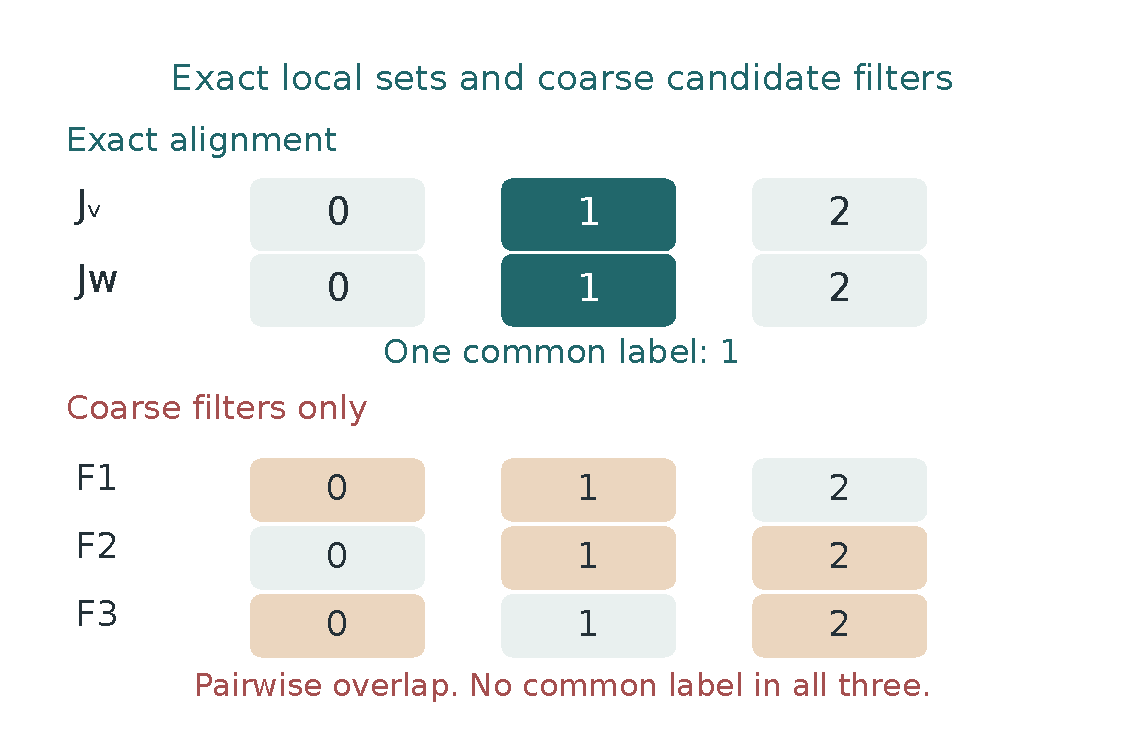
\includegraphics[width=.90\linewidth]{10_alignment.pdf}
\caption{Exact alignment requires one common global label. The upper rows give exact local sets. The lower rows are coarse filters, which need a separate intersection test.}
\label{fig:global_alignment}\end{figure}

\section{Every descent of an Artin base change is locally Artin}\label{sec:local_artin}

The automorphic descent has much stronger local structure than a general cusp form.

\begin{theorem}[Local Artin descent]\label{thm:local_artin_descent}
Let \(E/F\) be a finite extension, let \(\pi\) be an automorphic representation of \(\GL_n(\Adele_F)\), and suppose its base change \(\Pi\) to \(E\) exists with local compatibility. Assume every local Weil Deligne parameter of \(\Pi\) has zero monodromy and finite Weil image. Then the same is true for every local parameter of \(\pi\).
\end{theorem}

\begin{proof}
Fix \(v\) and \(w\mid v\), and write the local Weil Deligne parameter as \((\phi_v,N_v)\). Base change restricts \(\phi_v\) to \(W_{E_w}\) and keeps the monodromy operator. Since the parameter of \(\Pi_w\) has zero monodromy, \(N_v=0\).

The image of \(W_{E_w}\) under \(\phi_v\) is finite. The subgroup \(W_{E_w}\) has finite index in \(W_{F_v}\). Choose finitely many coset representatives. The full image \(\phi_v(W_{F_v})\) is contained in the union of the corresponding finitely many cosets of the finite subgroup \(\phi_v(W_{E_w})\). Hence it is finite.
\end{proof}

\begin{corollary}[Tempered local descent]\label{cor:tempered_local_descent}
Under the hypotheses of \cref{thm:local_artin_descent}, every local parameter is bounded. Thus every local component of \(\pi\) is tempered in the normalized local Langlands correspondence.
\end{corollary}

\begin{proof}
A finite subgroup of \(\GL_n(\CC)\) is bounded. Local Langlands for general linear groups identifies bounded parameters with tempered representations \cite{Henniart2000}.
\end{proof}

\begin{corollary}[Artin infinity type]\label{cor:artin_infinity}
If the base change is attached to a finite image global Galois representation, every archimedean local parameter of the descent has finite image.
\end{corollary}

\begin{proof}
Apply \cref{thm:local_artin_descent} at the archimedean Weil groups. The subgroup corresponding to the extension has finite index.
\end{proof}

\section{Finite Satake descent}\label{sec:finite_satake}

Let \(E/F\) be a finite Galois extension of degree \(d\). Suppose \(\pi\) base changes to an automorphic representation \(\Pi\) attached to a finite image Artin representation \(\tau\). Let \(M\) be the exponent of the finite image of \(\tau\). Fix a finite set \(S\) containing the exceptional comparison places and all ramification of the extension and the representations. The unramified conclusions in this section refer to places outside this fixed set. Weak attachment over the extension field suffices for these conclusions. If all local attachment over the extension field is known, the preceding local finiteness theorem supplies the stronger conclusion at every place.

\begin{theorem}[Finite Satake roots]\label{thm:finite_satake_roots}
At every finite place \(v\) where \(E/F\), \(\pi\), and \(\Pi\) are unramified and the stated Artin polynomial comparison holds above \(v\), every normalized Satake root of \(\pi_v\) belongs to
\[
 \boxed{
 \mu_{dM}.
 }
\]
\end{theorem}

\begin{proof}
Choose \(w\mid v\) and let \(f=f(w/v)\). If the normalized Satake roots of \(\pi_v\) are \(\alpha_1,\ldots,\alpha_n\), unramified base change replaces the Satake conjugacy class by its \(f\)th power. Hence the roots of \(\Pi_w\) are \(\alpha_i^f\). Since \(\Pi_w\) is attached to a representation of exponent dividing \(M\),
\[
 (\alpha_i^f)^M=1.
\]
Thus \(\alpha_i\in\mu_{fM}\). Since \(f\mid d\), this group is contained in \(\mu_{dM}\).
\end{proof}

\begin{corollary}[Integral Hecke polynomials]\label{cor:integral_hecke}
Every normalized Hecke polynomial of \(\pi\) at a place outside the fixed exceptional set \(S\) has coefficients in
\[
 \boxed{
 \ZZ[\mu_{dM}].
 }
\]
In particular, all of its coefficients are algebraic integers.
\end{corollary}

\begin{proof}
The coefficients are elementary symmetric polynomials in roots of unity from \(\mu_{dM}\).
\end{proof}

\begin{corollary}[Finite Hecke field]\label{cor:finite_hecke_field}
The field generated by the normalized Hecke coefficients of \(\pi\) outside \(S\) is a number field contained in
\[
 \boxed{
 \QQ(\mu_{dM}).
 }
\]
There are only finitely many possible normalized Hecke polynomials of degree \(n\) at these places.
\end{corollary}

\begin{proof}
Every coefficient belongs to the fixed cyclotomic field by \cref{cor:integral_hecke}. Every root lies in the finite set \(\mu_{dM}\), so only finitely many multisets of \(n\) roots, and therefore only finitely many Hecke polynomials, can occur.
\end{proof}

\begin{corollary}[Finite order central character]\label{cor:finite_central_char}
The central character of \(\pi\) has finite order.
\end{corollary}

\begin{proof}
Outside the fixed exceptional set, every unramified determinant value lies in \(\mu_{dM}\). The Hecke character \(\omega_\pi^{dM}\) is therefore trivial at every unramified place outside a finite set. The one dimensional strong multiplicity one statement, or equivalently uniqueness of a Hecke character from its almost everywhere unramified values, makes it the trivial global character. Thus \(\omega_\pi\) has finite order. This argument does not require a separate local finiteness assertion at an exceptional place.
\end{proof}

\begin{definition}[Finite Satake cusp form]\label{def:finite_satake_cusp}
A cuspidal representation of \(\GL_n(\Adele_F)\) is finite Satake when, outside one finite exceptional set, its normalized unramified Satake roots lie in one finite subgroup of \(\CC^\times\). The exceptional set is fixed, not allowed to change separately for each coefficient or prime.
\end{definition}

\begin{corollary}[Cyclic Artin descent is finite Satake]\label{cor:cyclic_finite_satake}
Every cuspidal cyclic descent of an automorphic Artin representation is finite Satake.
\end{corollary}

\begin{proof}
Apply \cref{thm:finite_satake_roots}.
\end{proof}


\subsection{Cyclotomic rigidity}

\begin{proposition}[Finite number of unramified Hecke polynomials]\label{prop:finite_number_hecke}
Under the hypotheses of \cref{thm:finite_satake_roots}, put \(N=dM\). The number of possible normalized Hecke polynomials of degree \(n\) outside \(S\) is at most
\[
 \boxed{
 \binom{N+n-1}{n}.
 }
\]
\end{proposition}

\begin{proof}
A polynomial is determined by the multiset of its \(n\) Satake roots. Those roots lie in the \(N\) element set \(\mu_N\). The number of multisets of size \(n\) selected from \(N\) elements is the displayed binomial coefficient.
\end{proof}

\begin{corollary}[Finite trace alphabet]\label{cor:finite_trace_alphabet}
The normalized Hecke traces of \(\pi\) outside \(S\) belong to a finite subset of \(\ZZ[\mu_{dM}]\).
\end{corollary}

\begin{proof}
Each trace is a sum of \(n\) roots from the fixed finite set \(\mu_{dM}\).
\end{proof}

\begin{corollary}[Unramified Ramanujan property]\label{cor:unramified_ramanujan}
Every normalized Satake root at the allowed unramified places has complex absolute value one.
\end{corollary}

\begin{proof}
Every root is a root of unity by \cref{thm:finite_satake_roots}.
\end{proof}


\section{Finite polynomial alphabets and separating primes}\label{sec:separating_primes}

Let \(K\) be a number field containing the normalized unramified Hecke coefficients of a finite Satake descent, the character values of the target Artin representation, and the values of the quotient character. Enlarge it to a splitting field in which the target and its restriction have matrix realizations. Let \(\OO_K\) be its ring of integers.

\begin{definition}[Finite polynomial alphabet]\label{def:finite_alphabet}
The finite polynomial alphabet of the cyclic attachment problem is the union
\[
\calA
=
\calA_{\pi}
\cup
\calA_{\rho},
\]
where \(\calA_{\pi}\) is the set of normalized Hecke polynomials occurring for \(\pi\) outside the fixed exceptional set, and \(\calA_{\rho}\) is the set of characteristic polynomials occurring for the finitely many twists
\[
\rho\otimes\epsilon^j,
\qquad
j\in\ZZ/p\ZZ.
\]
\end{definition}

\begin{proposition}[Finiteness of the alphabet]\label{prop:finite_alphabet}
The set \(\calA\) is finite and is contained in \(\OO_K[T]\).
\end{proposition}

\begin{proof}
The descent alphabet is finite by \cref{thm:finite_satake_roots,prop:finite_number_hecke}. The Artin image and the quotient twist group are finite, so only finitely many characteristic polynomials occur on that side. Every root is a root of unity, so every coefficient is an algebraic integer.
\end{proof}

\begin{definition}[Separating coefficient prime]\label{def:separating_prime}
A finite place \(\lambda\) of \(K\) is separating for \(\calA\) when reduction modulo \(\lambda\) is injective on \(\calA\).
\end{definition}

\begin{theorem}[Existence of separating primes]\label{thm:separating_primes}
All but finitely many finite places of \(K\) are separating for \(\calA\).
\end{theorem}

\begin{proof}
For every ordered pair of distinct polynomials \(P,Q\in\calA\), choose one nonzero coefficient difference. Only finitely many finite places divide one of these finitely many nonzero algebraic integers. Outside their union, no two polynomials have the same reduction.
\end{proof}

\begin{lemma}[Good reduction of an absolutely irreducible finite representation]\label{lem:good_irreducible_reduction}
Let \(\tau\) be an absolutely irreducible representation of a finite group over a number field \(K\). In a fixed matrix realization, exclude the finitely many coefficient places at which a group matrix has a denominator. The resulting stable local lattices have absolutely irreducible reduction at all but finitely many further places.
\end{lemma}

\begin{proof}
Absolute irreducibility and Burnside's theorem give group elements \(g_1,\ldots,g_{n^2}\) whose matrices form a \(K\) basis of \(M_n(K)\). Vectorize these matrices in the fixed basis. Their determinant is nonzero. Exclude places at which that determinant is zero or has a denominator, together with denominators of the finitely many group matrices. At a remaining place the coordinate lattice is stable, and the reduced matrices span the full matrix algebra over the residue field. They continue to span it after extending the residue field. Any invariant subspace is then invariant under every matrix, so it is zero or the full space. This proves absolute irreducibility of the reduction. The argument is local at the good places and does not require a globally free integral lattice over \(\OO_K\).
\end{proof}

\begin{definition}[Good separating prime]\label{def:good_separating_prime}
A finite place \(\lambda\) is good for the cyclic attachment problem when

\begin{enumerate}
\item it is separating for \(\calA\)
\item its residue characteristic is different from \(p\)
\item the reduction of \(\tau=\rho|_{G_E}\) is absolutely irreducible.
\end{enumerate}
\end{definition}

\begin{corollary}[Abundance of good primes]\label{cor:abundant_good_primes}
All but finitely many finite places of \(K\) are good.
\end{corollary}

\begin{proof}
Combine \cref{thm:separating_primes,lem:good_irreducible_reduction} and exclude the finitely many places above \(p\).
\end{proof}

\section{Finite trace alphabets in residual characteristic}\label{sec:finite_trace_bound}

The next theorem gives an explicit bound for a finite residual image using only its trace alphabet.

\begin{theorem}[Finite trace image bound]\label{thm:finite_trace_image_bound}
Let \(k\) be algebraically closed of characteristic zero or characteristic \(\ell>n\). Let \(\Gamma\subseteq\GL_n(k)\) be a subgroup, and assume its defining module \(k^n\) is semisimple. Suppose its trace set is finite, with
\[
 t=\#\{\Tr(\gamma):\gamma\in\Gamma\}.
\]
Then \(\Gamma\) is finite and
\[
 \abs\Gamma\le t^{\dim_k A}\le t^{n^2},
 \qquad A=\operatorname{span}_k\Gamma.
\]
In particular this bounds a finite semisimple residual matrix group in characteristic greater than its rank.
\end{theorem}

\begin{proof}
Because products of group matrices are group matrices, \(A\) is a finite dimensional subalgebra of \(M_n(k)\). An \(A\) submodule is the same thing as a \(\Gamma\) submodule. The given module is semisimple and faithful for \(A\). The Jacobson radical annihilates every simple constituent, hence annihilates this faithful module. It is therefore zero. The split semisimple algebra has the form
\[
 A\cong\bigoplus_iM_{d_i}(k),\qquad
 k^n\cong\bigoplus_i(k^{d_i})^{\oplus m_i},
 \qquad\sum_i d_im_i=n.
\]
Faithfulness gives \(m_i\ge1\) for every block. The trace pairing
\[
 B(x,y)=\Tr_{k^n}(xy)
\]
restricts on the \(i\)th block to \(m_i\Tr(XY)\). Matrix trace pairing is nondegenerate, as is seen by pairing matrix units \(E_{ab}\) with \(E_{ba}\). Each \(m_i\) is nonzero in \(k\): this is automatic in characteristic zero, and follows from \(1\le m_i\le n<\ell\) in residual characteristic. Thus \(B\) is nondegenerate on \(A\).

Choose a basis \(\gamma_1,\ldots,\gamma_r\) of \(A\) from the spanning set \(\Gamma\), where \(r=\dim_k A\le n^2\). Send an image element to
\[
 \Phi(\gamma)=\bigl(\Tr(\gamma\gamma_1),\ldots,
                         \Tr(\gamma\gamma_r)\bigr).
\]
All coordinates lie in the trace set, because \(\gamma\gamma_i\in\Gamma\). If two tuples agree, then \(\gamma-\gamma'\) pairs to zero with every basis element, hence every element of \(A\). Nondegeneracy gives \(\gamma=\gamma'\). Therefore \(\Phi\) injects \(\Gamma\) into a set of size \(t^r\). This proves finiteness as well as the bound. Prior finiteness of \(\Gamma\) was not needed in this argument.
\end{proof}

\begin{figure}[tbp]\centering
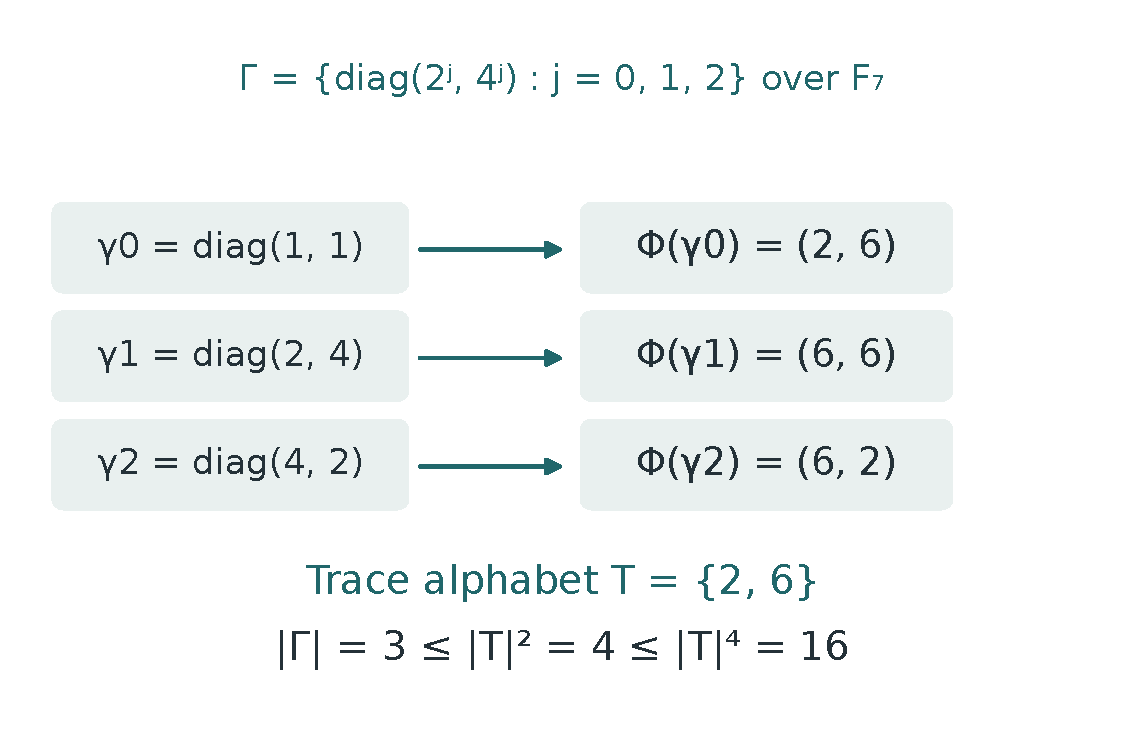
\includegraphics[width=.90\linewidth]{14_trace_bound.pdf}
\caption{The nondegenerate trace pairing records each image element by finitely many traces of products with basis elements. This gives an injective encoding by the finite alphabet.}
\label{fig:trace_alphabet_bound}\end{figure}

\begin{remark}[Historical position of the trace bound]\label{rem:trace_bound_history}
The proof is elementary once the semisimple image algebra and its trace pairing are written down. No claim of historical priority is made. The theorem should be compared with modular Jordan type bounds and with the literature on finite trace sets in Galois representations.
\end{remark}

\begin{corollary}[Uniform bound for a residual Galois image]\label{cor:residual_image_bound}
Let
\[
 \overline r:G_F\longrightarrow\GL_n(\overline\FF_{\ell})
\]
be continuous and semisimple, with \(\ell>n\). If its Frobenius traces belong to a set of size at most \(t\) on a Chebotarev dense set, then
\[
\boxed{
 \abs{\im\overline r}\leq t^{n^2}.
}
\]
\end{corollary}

\begin{proof}
Continuity gives finite image. Chebotarev shows that every conjugacy class of the finite image occurs as an unramified Frobenius class. Apply \cref{thm:finite_trace_image_bound}.
\end{proof}

\begin{standardfact}[Cross characteristic lifting]\label{fact:cross_characteristic_lifting}
Let \(\Gamma\) be finite and let \(\ell\nmid\abs\Gamma\). Every semisimple representation of \(\Gamma\) over an algebraically closed field of characteristic \(\ell\) is the reduction of a characteristic zero representation after a finite extension of coefficient fields. Irreducible representations lift to irreducible representations, and characteristic polynomials reduce compatibly. This is the nonmodular case of Brauer character theory \cite{BrauerNesbitt1941,CurtisReiner1962,Serre1977}.
\end{standardfact}

\begin{definition}[Universal bounded cyclotomic alphabet]\label{def:bounded_cyclotomic_alphabet}
For positive integers \(n\) and \(B\), let \(\calQ_{n,B}\) be the finite set of monic degree \(n\) polynomials whose roots are roots of unity of order at most \(B\).
\end{definition}

\begin{theorem}[One large residual realization gives an Artin representation]\label{thm:large_residual_realization}
Let \(K\) be a number field, let \(S\) be a finite set of places of \(F\), and let \(\calP\subseteq\OO_K[T]\) be a nonempty finite set of monic degree \(n\) polynomials. Assume all their roots are roots of unity. For \(v\notin S\), choose \(P_v\in\calP\).

There is a finite set \(\Sigma(\calP)\) of rational primes, fixed from the alphabet before any realization is chosen, with the following property. Let \(\lambda\) be a coefficient place whose residue characteristic \(\ell\) is outside \(\Sigma(\calP)\). Suppose a continuous semisimple representation
\[
 \overline r_\lambda:G_F\longrightarrow\GL_n(\overline\FF_\ell)
\]
is unramified outside \(S\) and the places above \(\ell\), and has characteristic polynomial \(\overline{P_v}\) at every remaining unramified place. Then there is a finite image semisimple complex representation \(r\) with polynomial \(P_v\) at those places. If \(\overline r_\lambda\) is absolutely irreducible, then \(r\) is irreducible.
\end{theorem}

\begin{proof}
Let \(t\ge1\) be the number of trace values in the source alphabet and put \(B=t^{n^2}\). First fix a finite normal extension \(L/\QQ\) containing \(K\) and the roots of unity of orders dividing
\[
 D_B=\operatorname{lcm}(1,2,\ldots,B).
\]
Every polynomial in \(\calQ_{n,B}\), the bounded cyclotomic alphabet, has coefficients in \(L\). Form the union of all Galois conjugates in \(L\) of \(\calP\cup\calQ_{n,B}\). This is a fixed finite set of integral polynomials. For each distinct pair choose one nonzero coefficient difference. Exclude the rational primes below the prime divisors of all these differences, and exclude the rational primes \(\ell\le\max(n,B)\). This defines a finite exceptional set independent of any residual representation or choice of lift. Outside it, reduction at every place of \(L\) above \(\ell\) is injective on this enlarged polynomial set.

Continuity of \(\overline r_\lambda\) into the discrete residual matrix group gives finite image \(\Gamma\). Every conjugacy class of that image occurs at unramified Frobenius places away from the finite excluded set by Chebotarev. Its trace set has size at most \(t\), because the Frobenius polynomials are reductions of the prescribed alphabet. \Cref{thm:finite_trace_image_bound} gives \(\abs\Gamma\le B<\ell\), so \(\ell\nmid\abs\Gamma\).

Use the cross characteristic lifting statement in \cref{fact:cross_characteristic_lifting}, in a splitting modular system compatible with the chosen coefficient place. It gives an ordinary characteristic zero representation of \(\Gamma\) whose reduction is the prescribed residual representation. Compose it with \(G_F\to\Gamma\). Each lifted eigenvalue has order dividing the order of an element of \(\Gamma\), hence at most \(B\). Every lifted Frobenius polynomial consequently belongs to \(\calQ_{n,B}\).

Only characteristic polynomials, not all matrix entries of the lift, are needed in the fixed separation field \(L\). The lift can be realized over a further number field and reduced at a compatible place above \(\lambda\). Its Frobenius polynomial and \(P_v\) have equal reduction there. On restriction to \(L\), injectivity of the fixed enlarged alphabet makes them equal in characteristic zero. The chosen compatible embedding fixes the specified copy of \(K\), so the equalities recover the original \(P_v\) simultaneously. The nonmodular correspondence preserves irreducibility. This proves the final assertion.
\end{proof}

\begin{corollary}[Large residual realization of a finite Satake cusp form]\label{cor:large_residual_finite_satake}
Let \(\pi\) be a finite Satake cuspidal representation whose normalized Hecke polynomials lie in \(K\). If one sufficiently large residual Galois realization with the expected unramified polynomials exists, then \(\pi\) has a finite image complex Galois realization. Absolute irreducibility of the residual realization gives an irreducible Artin representation.
\end{corollary}

\begin{proof}
Apply \cref{thm:large_residual_realization} to the finite Hecke polynomial alphabet of \(\pi\).
\end{proof}

\section{One prime residual attachment}\label{sec:one_prime_attachment}

\begin{definition}[Residual realization of a descent]\label{def:residual_realization}
Let \(\lambda\) be a finite place of the coefficient field. A residual realization of \(\pi\) at \(\lambda\) is a continuous semisimple representation
\[
\overline r_{\pi,\lambda}:G_F\longrightarrow\GL_n(\overline k_{\lambda})
\]
whose characteristic polynomial at every unramified place outside a finite set is the reduction of the normalized Hecke polynomial of \(\pi\).
\end{definition}

\begin{theorem}[One prime residual attachment]\label{thm:one_prime_attachment}
Use the cyclic Artin setup of \cref{def:attached_descent}. For this unramified theorem it is enough that the lower cuspidal representation \(\Pi\) is weakly attached to \(\tau\), with \(\pi\) a cuspidal cyclic descent. Let \(\lambda\) be a good separating prime. Suppose \(\pi\) has a residual realization \(\overline r_{\pi,\lambda}\). Then there is a unique index
\[
j_{\lambda}\in\ZZ/p\ZZ
\]
such that
\[
\boxed{
P_{\pi,v}(T)
=
P_{\rho\otimes\epsilon^{j_{\lambda}},v}(T)
}
\]
for every finite place \(v\) outside a finite set. Consequently,
\[
\pi\otimes\epsilon^{-j_{\lambda}}
\]
is weakly attached to \(\rho\).
\end{theorem}

\begin{proof}
Restrict the residual realization to \(G_E\). At every unramified place \(w\) of \(E\) above a good place \(v\) of \(F\), cyclic base change identifies the characteristic polynomial of the restriction with the reduction of the Hecke polynomial of \(\Pi_w\). Since \(\Pi\) is attached to \(\tau\), this is the characteristic polynomial of \(\overline\tau(\Frob_w)\). Chebotarev density and Brauer Nesbitt give
\[
\left(
\overline r_{\pi,\lambda}|_{G_E}
\right)^{\mathrm{ss}}
\cong
\overline\tau.
\]
The right side is absolutely irreducible and has the full dimension \(n\). Hence the restriction itself has one composition factor and is irreducible, so it is isomorphic to \(\overline\tau\).

The representations \(\overline r_{\pi,\lambda}\) and \(\overline\rho\) are therefore two extensions of the same absolutely irreducible representation of \(G_E\). Their ratio is a character of \(G_F/G_E\). Since the residue characteristic is different from \(p\), the reduced quotient character has order \(p\), and there is a unique index \(j_{\lambda}\) with
\[
\overline r_{\pi,\lambda}
\cong
\overline\rho\otimes\overline\epsilon^{j_{\lambda}}.
\]
At every good unramified place,
\[
P_{\pi,v}
\equiv
P_{\rho\otimes\epsilon^{j_{\lambda}},v}
\pmod\lambda.
\]
Both polynomials belong to the finite alphabet \(\calA\). The prime is separating, so the congruence is equality in characteristic zero. Uniqueness follows from the freeness of the extension torsor.
\end{proof}

\begin{corollary}[Only finitely many local checks remain]\label{cor:finitely_many_local_checks}
Under \cref{thm:one_prime_attachment}, all local attachment to \(\rho\) is equivalent to checking the label \(-j_\lambda\) at every exceptional finite place excluded from the unramified comparison and at every archimedean place.
\end{corollary}

\begin{proof}
At the unramified places covered by the theorem, equality of the semisimple characteristic polynomials identifies the local parameters. At each remaining finite or archimedean place, use the corresponding local attachment condition. There are finitely many such places. When the stronger all local setup over the extension field holds, the finite image local parameters at a cyclic quotient are compared by the exact extension spectrum criterion, and the split restrictions already give equality. Under only lower weak attachment, the exceptional local comparison is a separate premise and finite local Artin type is not inferred there. These checks include the infinity parameters and any exceptional unramified place, rather than just the ramified places.
\end{proof}

\begin{corollary}[Infinitely many residual realizations suffice]\label{cor:infinitely_many_residual}
If residual realizations of \(\pi\) exist at infinitely many coefficient places, then one of them is good, and \(\pi\) is weakly attached after one quotient twist.
\end{corollary}

\begin{proof}
Only finitely many coefficient places are not good by \cref{cor:abundant_good_primes}. Apply \cref{thm:one_prime_attachment} at any good place carrying a residual realization.
\end{proof}

\begin{corollary}[A congruent cohomological eigensystem suffices]\label{cor:congruent_cohomological}
Let \(\lambda\) be good. Suppose the reduction of the Hecke eigensystem of \(\pi\) occurs in a setting that supplies a semisimple residual Galois representation with the expected unramified characteristic polynomials. Then the conclusion of \cref{thm:one_prime_attachment} holds.
\end{corollary}

\begin{proof}
The supplied representation is a residual realization in the sense of \cref{def:residual_realization}.
\end{proof}

\section{Representation theoretic collapse at the quotient prime}\label{sec:residual_collapse}

Let \(K\) be a number field containing the values of the order \(p\) quotient characters, let \(\lambda_p\) be a place above \(p\), and let \(\OO\) be the corresponding valuation ring.

\begin{theorem}[Semisimple collapse of cyclic extension labels]\label{thm:semisimple_label_collapse}
Let \(G\) be finite, let \(H\triangleleft G\) with \(G/H\cong C_p\), and let \(V,W\) be semisimple representations over a number field \(K\) with isomorphic restrictions to \(H\). Choose stable lattices at a coefficient place above \(p\). Over an algebraic closure of the residue field their semisimplified reductions satisfy
\[
 \overline V^{\mathrm{ss}}\cong\overline W^{\mathrm{ss}}.
\]
The same statement applies to finite image representations of an arbitrary group after passing to a common finite quotient that retains the cyclic quotient.
\end{theorem}

\begin{proof}
For \(g\in G\), write its commuting primary decomposition as \(g=g_p g_s\), where \(g_p\) has \(p\) power order and \(g_s\) has order prime to \(p\). The image of \(g_s\) in \(C_p\) is trivial, so \(g_s\in H\). In residue characteristic \(p\), the matrix of \(g_s\) is diagonalizable after extending the field, and the matrix of \(g_p\) is unipotent. They commute, so the latter preserves each eigenspace of the former. On an eigenspace with eigenvalue \(\alpha\), the product is \(\alpha\) times a unipotent operator. Its characteristic polynomial has only the root \(\alpha\), with that eigenspace's dimension as multiplicity. Therefore the reduced characteristic polynomials of \(g\) and \(g_s\) agree.

The restrictions of \(V,W\) agree on \(H\), so their reduced characteristic polynomials agree at \(g_s\), hence at every \(g\). The classical modular Brauer Nesbitt theorem identifies the semisimplifications over the algebraic closure of the residue field \cite{BrauerNesbitt1941,Chenevier2014}. We use its full characteristic polynomial form, valid in arbitrary residual characteristic. Chenevier's checked preprint Theorem A, Lemma 1.12(ii), and Theorem 2.12 give the determinant and uniqueness interface. No restriction \(p>n\) is needed for this uniqueness assertion. This proof does not assume that the original number field is a splitting field, or choose stable type extensions over it. For finite image representations of a larger group, quotient by the intersection of their kernels with \(H\). The resulting finite quotient has the same argument.
\end{proof}

\begin{corollary}[Residual collapse in the global and local fibres]\label{cor:two_torsor_residual_collapse}
At a coefficient prime above the cyclic degree \(p\), all global Galois extensions of a fixed irreducible restriction have the same semisimplified reduction. At any one place, local parameters with the same restricted finite image parameter have the same semisimplified reduction after passing to a common finite local quotient and compatible coefficient field.
\end{corollary}

\begin{proof}
Apply \cref{thm:semisimple_label_collapse} in the global finite quotient for the first assertion, and in the common local finite quotient for the second. The comparison is always between representations of the same group. In the cyclic descent setup the required local restriction equality is supplied by full local base change compatibility and attachment over the extension field.
\end{proof}

\section{The quotient prime residual congruence}\label{sec:quotient_prime}

Let \(\lambda_p\) be a finite place of the coefficient field above the cyclic degree \(p\), chosen after adjoining the values of the quotient character. Then
\[
\epsilon\equiv1\pmod{\lambda_p}.
\]

\begin{definition}[Frobenius transform of a polynomial]\label{def:frobenius_transform}
If
\[
P(T)=\prod_{i=1}^{n}(T-\alpha_i),
\]
define
\[
P^{[p]}(T)
=
\prod_{i=1}^{n}(T-\alpha_i^p).
\]
This is a polynomial expression in the coefficients of \(P\).
\end{definition}

\begin{lemma}[Frobenius transform after reduction]\label{lem:frobenius_transform}
Let \(P\) have integral coefficients at a place of residue characteristic \(p\). Then
\[
\boxed{
\overline{P^{[p]}}(T)
=
\operatorname{Frob}\bigl(\overline P(T)\bigr),
}
\]
where Frobenius raises every coefficient to its \(p\)th power. In particular, the map
\[
\overline P\longmapsto\overline{P^{[p]}}
\]
is injective over the residue field.
\end{lemma}

\begin{proof}
Over an algebraic closure of the residue field,
\[
\overline{P^{[p]}}(T)
=
\prod_i(T-\overline\alpha_i^p).
\]
The elementary symmetric functions of the \(p\)th powers are the \(p\)th powers of the elementary symmetric functions in characteristic \(p\). Finite residue fields are perfect, so Frobenius is injective.
\end{proof}

\begin{theorem}[Canonical quotient prime congruence]\label{thm:quotient_prime_congruence}
Use the cyclic Artin setup of \cref{def:attached_descent}. For every finite place \(v\) outside a finite set,
\[
\boxed{
P_{\pi,v}(T)
\equiv
P_{\rho,v}(T)
\pmod{\lambda_p}.
}
\]
Thus the semisimplified reduction of \(\rho\) is residually automorphic with the mod \(\lambda_p\) Hecke eigensystem of every cuspidal descent of \(\Pi\).
\end{theorem}

\begin{proof}
Assume first that \(v\) splits in \(E\). Local base change is the identity at every place above \(v\), so the two polynomials agree before reduction.

Assume that \(v\) is unramified and nonsplit. Since the extension has prime degree, its residue degree is \(p\). Unramified base change raises the Satake conjugacy class of \(\pi_v\) to its \(p\)th power. Restriction of \(\rho_v\) to \(W_{E_w}\) does the same to its Frobenius class. Since \(\Pi_w\) is attached to \(\rho|_{W_{E_w}}\),
\[
P_{\pi,v}^{[p]}(T)
=
P_{\rho,v}^{[p]}(T).
\]
Reduce modulo \(\lambda_p\) and use \cref{lem:frobenius_transform}. Injectivity of residue Frobenius gives the desired congruence. The finitely many ramified and excluded places do not affect residual attachment.
\end{proof}

\begin{corollary}[All cyclic twists collapse residually]\label{cor:twists_collapse_residually}
For every \(j\in\ZZ/p\ZZ\),
\[
\overline{\rho\otimes\epsilon^j}
\cong
\overline\rho
\]
at the semisimple character level modulo \(\lambda_p\). Likewise, all automorphic descents have the same mod \(\lambda_p\) unramified Hecke eigensystem.
\end{corollary}

\begin{proof}
The values of \(\epsilon\) are \(p\)th roots of unity and reduce to one at \(\lambda_p\). Apply \cref{thm:quotient_prime_congruence} to every descent twist.
\end{proof}

\begin{definition}[Quotient prime lifting gate]\label{def:quotient_prime_lifting}
The quotient prime lifting gate is the assertion that the matching residual unramified eigensystems supplied by \cref{thm:quotient_prime_congruence}, together with the local deformation conditions of \(\rho\), lift to characteristic zero automorphy of \(\rho\).
\end{definition}

\begin{theorem}[Quotient prime reduction of a cyclic step]\label{thm:quotient_prime_reduction}
If the quotient prime lifting gate holds for the cyclic step, then the target representation \(\rho\) is automorphic. Hence Strong Artin for all finite solvable images follows if this gate holds at every invariant extension step of every solvable Clifford tower.
\end{theorem}

\begin{proof}
The residual polynomial input is \cref{thm:quotient_prime_congruence}. The first conclusion is the definition of the lifting gate. The second follows by the Clifford recursion in \cref{cor:clifford_reduction}.
\end{proof}

\begin{remark}\label{rem:quotient_prime_difficulty}
The quotient prime often divides the residual image order, and the resulting residual representation can be nonadequate or nonregular. The congruence theorem supplies matching residual unramified eigensystems. It does not supply the required weight raising, local component control, or nonregular automorphy lifting theorem.
\end{remark}

\section{Finite Satake rigidity for l adic realizations}\label{sec:ladic_rigidity}

\begin{theorem}[Finite Frobenius trace rigidity]\label{thm:finite_trace_ladic_rigidity}
Let \(L/\QQ_\ell\) be finite and let \(r:G_F\to\GL_n(L)\) be continuous, semisimple, and unramified outside a finite set. Suppose its traces at a density one set of unramified places belong to one finite set \(T\), of size \(t\). Then
\[
 \abs{r(G_F)}\le t^{n^2}.
\]
In particular \(r\) has finite image.
\end{theorem}

\begin{proof}
The image is compact. Choose a stable integral lattice after conjugation, so reductions modulo successive powers of a uniformizer give finite quotient images. Fix \(g\in G_F\) and one such quotient. The Chebotarev class of the image of \(g\) has positive density. A density one set meets it, even after removing the finite set of ramified places. Thus some selected Frobenius matrix is conjugate to the image of \(r(g)\) modulo that power, and their traces are congruent.

For each precision, \(\Tr r(g)\) is therefore arbitrarily close to an element of \(T\). The finite set \(T\) is closed in \(L\), so \(\Tr r(g)\in T\). Equivalently, one value in \(T\) occurs along an unbounded sequence of precisions, and its distance from \(\Tr r(g)\) tends to zero. This uses conjugacy classes, which suffice because trace is conjugacy invariant. It does not require choosing a preferred Frobenius element inside each class.

Extend scalars to an algebraic closure of \(L\). Semisimplicity is preserved in characteristic zero: the finite dimensional semisimple image algebra is separable. Apply the characteristic zero case of \cref{thm:finite_trace_image_bound} to \(\Gamma=r(G_F)\). Its faithful defining representation is semisimple and its trace set has size at most \(t\). This gives the stated bound directly, without an additional monodromy or torus argument.
\end{proof}

\begin{corollary}[Cyclotomic Frobenius rigidity]\label{thm:cyclotomic_ladic_rigidity}
Let \(r\) be as in \cref{thm:finite_trace_ladic_rigidity}. If every Frobenius eigenvalue on a density one set belongs to one fixed finite group \(\mu_N\), then \(r\) has finite image.
\end{corollary}

\begin{proof}
The Frobenius traces belong to the finite set of sums of \(n\) members of \(\mu_N\). Apply \cref{thm:finite_trace_ladic_rigidity}.
\end{proof}

\begin{theorem}[One semisimple l adic realization is enough]\label{thm:one_ladic_realization}
Let \(\pi\) be a finite Satake cuspidal representation with algebraic unramified Hecke polynomials. Fix an embedding of their number field into \(\overline\QQ_\ell\). Suppose there is a continuous semisimple representation \(r:G_F\to\GL_n(L)\), for a finite extension \(L/\QQ_\ell\), unramified outside a finite set, whose Frobenius polynomials agree with the embedded Hecke polynomials at almost all places. Then \(r\) has finite image and determines a finite image complex representation weakly attached to \(\pi\).
\end{theorem}

\begin{proof}
Finite Satake gives a finite set of embedded Frobenius traces. \Cref{thm:finite_trace_ladic_rigidity} makes the image finite. A characteristic zero representation of a finite group has cyclotomic character values and can be realized over an algebraic number field after choosing a splitting field. Choose the ordinary complex realization in a modular system compatible with the fixed embedding of the Hecke field. Characteristic polynomials then give the same algebraic polynomials under the two embeddings, so the complex representation is weakly attached to \(\pi\).

The assertion is about a globally semisimple representation. Frobenius semisimplicity alone is not substituted for that hypothesis. If an available construction supplies a representation not stated to be semisimple, its continuous semisimplification may be used when it has the same required unramified polynomials and finite ramification. The theorem then proves finite image of that semisimplification, not automatically of the original representation with extension data.
\end{proof}

\begin{corollary}[Finite Satake forms in existing realization ranges]\label{cor:existing_realization_ranges}
In every automorphic setting that supplies the continuous semisimple, finitely ramified realization required by \cref{thm:one_ladic_realization}, finite Satake implies an Artin realization.
\end{corollary}

\begin{proof}
Use \cref{thm:one_ladic_realization}.
\end{proof}

\section{Cohomological and weight raising realization gates}\label{sec:cohomological_gates}

\begin{standardfact}[A torsion cohomology realization range]\label{fact:scholze_torsion}
Scholze's Corollary 5.4.3 supplies a unique continuous semisimple residual representation for a Hecke eigensystem actually occurring in the stated cohomology of a locally symmetric space, under the field, level, coefficient, and theorem dependencies of that source \cite{Scholze2015}. The specified polynomial has coefficients \(q_v^{i(n+1)/2}T_{i,v}\), rather than an unspecified normalization of the eigenvalues. A fully stated unconditional subrange uses a CM field containing an imaginary quadratic field and the stated compatible set of rational primes. The more general totally real or CM formulation in the original article records stabilization dependencies. A determinant over a coefficient ring modulo a bounded nilpotent ideal and an actual residual representation are distinct outputs. For the gate here we require the latter and an explicit identification with our reduced normalized Hecke polynomials.
\end{standardfact}

\begin{standardfact}[A holomorphic limit realization range]\label{fact:goldring_shin}
Goldring's theorem, with an appendix by Shin, treats a unitary similitude group from a simple unitary Kottwitz datum and a cuspidal representation whose infinity component is an \(X\) holomorphic limit of discrete series \cite{GoldringShin2014}. At a coefficient prime satisfying the good reduction and reflex field conditions, it supplies a semisimple l adic representation over the CM field. Its local compatibility is stated on the density one split prime set with the twist \(\lvert\cdot\rvert^{(1-n)/2}\) in the source normalization. This is a concrete realization range. It is not a theorem for every singular infinity type or every finite Satake representation of \(\GL_n\).
\end{standardfact}

\begin{corollary}[A normalized torsion realization closes the weak step]\label{cor:scholze_attachment}
Use the cyclic Artin setup and a good separating prime \(\lambda\). Suppose the reduced eigensystem of a descent occurs in the cohomology range of \cref{fact:scholze_torsion}, with all source hypotheses met, and an explicit normalization comparison identifies the source Frobenius polynomials with \(\overline{P_{\pi,v}}\). Then the cyclic step is weakly attached after one quotient twist.
\end{corollary}

\begin{proof}
The declared occurrence, source theorem, and normalization comparison supply exactly the residual realization required by \cref{thm:one_prime_attachment}. No occurrence or normalization is inferred merely from finite Satake data.
\end{proof}

\begin{corollary}[A normalized holomorphic limit realization is finite image]\label{cor:goldring_shin_artin}
Suppose the representation supplied in \cref{fact:goldring_shin} is continuous, semisimple, and finitely ramified as in that source. Suppose further that a specified comparison identifies its density one split prime Frobenius polynomials with one fixed cyclotomic alphabet from the target normalized finite Satake data. Then that Galois representation has finite image.
\end{corollary}

\begin{proof}
The explicit comparison gives a finite trace alphabet on the density one set covered by the source's local compatibility. Apply \cref{thm:finite_trace_ladic_rigidity}. The normalization and density condition are essential premises. This corollary does not assert all local attachment or an arbitrary transfer from \(\GL_n\) into the unitary setting.
\end{proof}

\begin{standardfact}[Parallel weight one examples]\label{fact:weight_one_companion}
Gee and Kassaei's companion construction is for a totally real field unramified at \(p>2\), with an irreducible modular residual representation satisfying the stated residual image and local distinct eigenvalue hypotheses. Their Artin consequence assumes the relevant modularity statement for every totally odd residual two dimensional representation and every coefficient prime \cite{GeeKassaei2013}. Dimitrov and Wiese construct a continuous semisimple residual representation from a parallel weight one Hilbert eigenform of prime to \(p\) level. Its trace and determinant data require the stated Hecke and diamond character normalization \cite{DimitrovWiese2020}. These theorems illustrate realization and weight one methods in their precise ranks and hypotheses. They do not supply residual representations or weight raising in arbitrary rank.
\end{standardfact}

\begin{remark}\label{rem:known_gate_examples}
These results demonstrate two ways to close the new gates. Torsion or coherent cohomology supplies a separating residual realization. Hasse invariant methods raise the quotient prime congruence to a setting where Galois representations and lifting theorems are available. Neither construction is presently known for every rank and every finite Satake descent.
\end{remark}

\subsection{A p adic family realization gate}

\begin{definition}[Pseudocharacter family gate]\label{def:pseudo_family_gate}
A pseudocharacter family gate for a finite Satake descent \(\pi\) consists of a reduced p adic analytic space \(X\), a closed point \(x\) valued in a finite extension of \(\QQ_\ell\), and a continuous dimension \(n\) characteristic zero pseudorepresentation over \(\mathcal O(X)\). It factors through the Galois group unramified outside one finite set, and its unramified characteristic polynomials specialize at \(x\) to the embedded Hecke polynomials of \(\pi\). We use a point and coefficient setting in which characteristic zero realization produces a continuous semisimple representation after a finite coefficient extension. The existence of this family and the occurrence of the specified point are part of the gate.
\end{definition}

\begin{theorem}[A pseudocharacter family closes finite Satake realization]\label{thm:pseudo_family_closes}
If a finite Satake descent has the pseudocharacter family gate of \cref{def:pseudo_family_gate}, then it has a finite image semisimple Galois realization with the prescribed almost everywhere polynomials.
\end{theorem}

\begin{proof}
Specialize at \(x\) and use characteristic zero pseudorepresentation theory in the declared coefficient setting \cite{Chenevier2014}. This gives a continuous semisimple representation over a finite extension of \(\QQ_\ell\), factoring through the stated finitely ramified quotient. Its Frobenius polynomials are the required specialization. Apply \cref{thm:one_ladic_realization}. Neither specialization nor rigidity constructs the analytic space, the Galois pseudorepresentation on it, or the point corresponding to the descent.
\end{proof}

\begin{corollary}[Eigenvariety interpolation criterion]\label{cor:eigenvariety_interpolation}
Suppose a finite Satake descent is a closed finite valued point on a p adic eigenvariety or completed Hecke space, and the point and Galois pseudorepresentation satisfy every coefficient, continuity, finite ramification, and specialization condition of \cref{def:pseudo_family_gate}. Then the descent has a finite image Galois realization. Interpolation from classical points may be a way to construct the pseudorepresentation, but density by itself is not a substitute for these conditions.
\end{corollary}

\begin{proof}
The interpolated pseudorepresentation is a pseudocharacter family gate. Apply \cref{thm:pseudo_family_closes}.
\end{proof}

\begin{remark}\label{rem:eigenvariety_boundary}
The formal specialization theorem is complete. The unresolved geometric problem is to place every finite Satake descent on a space carrying such a pseudorepresentation. Weight one and holomorphic limit constructions prove this in important low weight settings, but no theorem presently covers every rank and every solvable cyclic descent.
\end{remark}

\section{A strengthened recursive Strong Artin theorem}\label{sec:strengthened_recursion}

\begin{definition}[Realization gate at an extension step]\label{def:realization_gate_step}
At an invariant cyclic extension step, a realization gate is any one of the following inputs for one cuspidal descent:

\begin{enumerate}
\item a residual realization at one good separating prime
\item a continuous semisimple finitely ramified l adic realization, including one obtained by a pseudocharacter family gate
\item a quotient prime weight raising and automorphy lifting theorem for the target Artin representation.
\end{enumerate}
\end{definition}

\begin{theorem}[Realization gates imply solvable Strong Artin]\label{thm:gates_imply_solvable_artin}
Let \(\rho\) be an irreducible finite image representation with solvable image. Follow it through a prime cyclic Clifford tower. Suppose every invariant extension step admits a realization gate in the sense of \cref{def:realization_gate_step}. Then \(\rho\) is weakly automorphic. If the remaining exceptional finite and archimedean local parameters align at every step, then the automorphic representation is attached at every place.
\end{theorem}

\begin{proof}
Begin with the one dimensional bottom representation and use class field theory. At an induction step, the distinct conjugate subgroup constituents give distinct automorphic conjugates by Chebotarev and strong multiplicity one. Prime cyclic automorphic induction therefore gives a cuspidal representation with the required almost everywhere parameters. At an invariant extension step, the lower cuspidal representation is Galois invariant because its conjugates have the same almost everywhere parameters as the invariant subgroup representation. Strong multiplicity one gives the invariance needed for cyclic descent. Choose a cuspidal descent. Lower weak attachment suffices for the finite Satake root bound outside a fixed finite set. The separate all local theorem retains its stronger local compatibility premise.

A separating residual realization gives the required characteristic zero quotient twist by \cref{thm:one_prime_attachment}. A sufficiently large residual realization gives a finite image complex representation by \cref{thm:large_residual_realization}. An l adic realization has finite image by \cref{thm:one_ladic_realization}. Its restriction is identified with the lower Artin representation by Chebotarev, so it lies in the extension torsor and one quotient twist selects the target. The quotient prime lifting gate gives the target directly by \cref{thm:quotient_prime_reduction}. Iteration gives weak automorphy at the top. The exceptional finite and archimedean local checks upgrade weak attachment to all place attachment by \cref{cor:finitely_many_local_checks}.
\end{proof}

\begin{corollary}[A single residual theorem target]\label{cor:single_residual_target}
The unramified form of Strong Artin for every finite solvable image would follow from a theorem supplying, at every cyclic extension step, one residual realization of a descent at one good separating coefficient prime.
\end{corollary}

\begin{proof}
Use the first realization gate in \cref{thm:gates_imply_solvable_artin}.
\end{proof}

\begin{corollary}[A single l adic theorem target]\label{cor:single_ladic_target}
The unramified form of Strong Artin for every finite solvable image would follow from a theorem supplying one continuous semisimple finitely ramified l adic realization for every finite Satake cuspidal descent.
\end{corollary}

\begin{proof}
Use the second realization gate in \cref{thm:gates_imply_solvable_artin}.
\end{proof}

\section{The weight zero realization bottleneck}\label{sec:realization}

The local finiteness theorem shows that the descended automorphic object already has the local shape of an Artin representation. The remaining problem is global realization.

\begin{standardfact}[Conditional construction of Kim and Yamauchi]\label{fact:kim_yamauchi}
Kim and Yamauchi's construction for \(\GL_n(\Adele_\QQ)\) uses five declared inputs: a finite Hecke field, integrality with a common denominator, cuspidal Galois conjugates, residual Galois realizations for all sufficiently large coefficient primes, and a Rankin Selberg coefficient bound obtainable from the required exterior power functoriality. Their theorem is a conditional construction of Artin representations, not a theorem producing the residual realizations for every weight zero cusp form \cite{KimYamauchi2016}. The finite alphabet and cross characteristic recovery below occupy closely related representation theoretic ground. Historical novelty is not inferred from their reformulation.
\end{standardfact}

\begin{theorem}[Automatic finite Satake inputs over the rational field]\label{thm:automatic_KY_inputs}
Let \(E/\QQ\) be finite Galois, and let \(\pi\) be a cuspidal representation of \(\GL_n(\Adele_\QQ)\) whose base change to \(E\) is attached to a finite image Artin representation. Then the following inputs in the Kim and Yamauchi strategy are automatic:

\begin{enumerate}
\item normalized Hecke polynomials outside the fixed exceptional set are integral
\item the normalized Hecke field away from that set is finite.
\end{enumerate}

The remaining hypotheses concern the global Galois realization, its conjugates, and the required exterior power functoriality.
\end{theorem}

\begin{proof}
The first two statements are \cref{cor:integral_hecke,cor:finite_hecke_field}. The description of the remaining inputs is the content of \cref{fact:kim_yamauchi}.
\end{proof}

\subsection{A complex pseudocharacter realization gate}

\begin{lemma}[Complex representations of profinite groups have finite image]\label{lem:complex_profinite_finite}
Let \(G\) be profinite and let \(r:G\to\GL_n(\CC)\) be continuous for the usual complex topology. Then \(r(G)\) is finite.
\end{lemma}

\begin{proof}
The Lie group \(\GL_n(\CC)\) has a neighborhood \(U\) of the identity that contains no nontrivial subgroup. Continuity gives a neighborhood \(r^{-1}(U)\) of the identity in \(G\). A profinite group has a basis of open normal subgroups, so one such subgroup \(N\) lies inside \(r^{-1}(U)\). Its image is a subgroup contained in \(U\), hence is trivial. Therefore \(r\) factors through the finite quotient \(G/N\). This proof uses a group neighborhood theorem. It does not use the false general topological assertion that an arbitrary continuous image of a totally disconnected space is totally disconnected.
\end{proof}

\begin{standardfact}[Characteristic zero pseudocharacters]\label{fact:pseudocharacter_realization}
Over an algebraically closed field of characteristic zero, a semisimple pseudocharacter of dimension \(n\) is the trace of a unique semisimple \(n\) dimensional representation up to isomorphism. We use this standard pseudocharacter realization principle in the form needed below \cite{Chenevier2014}.
\end{standardfact}

\begin{theorem}[Complex pseudocharacter gate]\label{thm:complex_pseudo_gate}
Let \(\pi\) be a finite Satake cuspidal representation of \(\GL_n(\Adele_F)\). Suppose there exists a continuous dimension \(n\) complex pseudocharacter \(T\) of \(G_F\), in the characteristic zero sense of \cref{fact:pseudocharacter_realization}, with characteristic polynomials at almost all unramified Frobenius classes equal to those of \(\pi\). Then \(\pi\) has a finite image semisimple Galois realization with those almost everywhere polynomials.
\end{theorem}

\begin{proof}
The algebraic pseudocharacter realization theorem supplies a semisimple representation \(r\) with trace \(T\). Its continuity deserves a separate argument. Let \(A\) be the span of its image. The trace pairing on \(A\) is nondegenerate, by the characteristic zero semisimple algebra argument in \cref{thm:finite_trace_image_bound}. Choose a basis \(r(g_1),\ldots,r(g_d)\) from the image. The functions
\[
 g\longmapsto\Tr(r(g)r(g_i))=T(gg_i)
\]
are continuous. Nondegeneracy says that these finitely many trace functions determine all linear coordinates of \(r(g)\) in \(A\). Inverting their fixed coefficient matrix proves that every matrix entry of \(r(g)\) is continuous. Now \cref{lem:complex_profinite_finite} gives finite image. The polynomial equality is the hypothesis. This continuity step is not silently supplied by the algebraic realization statement alone.
\end{proof}

\begin{corollary}[Pseudocharacter form of the realization bottleneck]\label{cor:pseudo_bottleneck}
For a finite Satake descent, constructing one continuous characteristic zero pseudocharacter with the prescribed Hecke polynomials is enough to produce the missing Artin representation.
\end{corollary}

\begin{proof}
Apply \cref{thm:complex_pseudo_gate}.
\end{proof}

\begin{definition}[Finite Satake realization principle]\label{def:finite_satake_principle}
The finite Satake realization principle asserts that a cuspidal representation of \(\GL_n(\Adele_F)\) with finite local Langlands image at every place and finite Satake data globally is attached to a finite image complex Galois representation.
\end{definition}

\begin{theorem}[Finite Satake realization implies solvable Strong Artin]\label{thm:FS_implies_solvable_artin}
Assume the finite Satake realization principle over every number field and in every rank. Then Strong Artin holds for every irreducible finite image Galois representation with solvable image.
\end{theorem}

\begin{proof}
Proceed up a prime cyclic Clifford tower. At an induction step, use automorphic induction. At an invariant extension step, the already automorphic restriction gives a Galois invariant cuspidal representation over the extension field. Cyclic base change descent supplies a cuspidal descent over the smaller field. By \cref{thm:local_artin_descent,cor:cyclic_finite_satake}, that descent satisfies the finite Satake realization principle, so it has a finite image Galois representation.

Base change of the realized representation has the same unramified Frobenius polynomials as \(\tau\). Chebotarev density and semisimplicity identify its restriction to \(G_E\) with \(\tau\). Since \(\tau\) is irreducible, the realized representation is irreducible and lies in the finite extension torsor. By \cref{prop:one_attachment}, twisting the automorphic descent by a quotient character selects the prescribed extension at that step. Iteration reaches the original representation.
\end{proof}

\begin{corollary}[A single new theorem target]\label{cor:single_target}
Strong Artin for all finite solvable images would follow from a global theorem realizing every finite Satake cuspidal representation as an Artin representation.
\end{corollary}

\begin{proof}
This is \cref{thm:FS_implies_solvable_artin}.
\end{proof}

\begin{remark}\label{rem:FS_scope}
The finite Satake realization principle is not proved here. It is a focused weight zero automorphic to Galois problem. The point of \cref{thm:FS_implies_solvable_artin} is that it replaces a separate attachment theorem at every solvable cyclic extension step by one global realization theorem.
\end{remark}

\section{A finite character separator on the Galois torsor}\label{sec:galois_separator}

The Galois extension torsor itself always admits a degree one separator.

\begin{theorem}[Trace separator for irreducible extensions]\label{thm:galois_trace_separator}
Let \(H\triangleleft G\) with \(G/H\cong C_p\), and let \(\rho\) be an irreducible extension of an irreducible \(G\) invariant representation of \(H\). Then there exists \(g\in G\setminus H\) such that
\[
 \boxed{
 \Tr\rho(g)\neq0.
 }
\]
Consequently, the \(p\) quotient twists of \(\rho\) are distinguished by their traces at \(g\).
\end{theorem}

\begin{proof}
The \(p\) extensions \(\rho\otimes\xi^j\) are pairwise nonisomorphic by \cref{prop:galois_torsor}. Their characters agree on \(H\). If \(\Tr\rho(g)=0\) for every \(g\notin H\), then all \(p\) characters would agree on every element of \(G\), contradicting their pairwise nonisomorphism. Thus some \(g\notin H\) has nonzero trace. At that element,
\[
 \Tr(\rho\otimes\xi^j)(g)
 =
 \xi(g)^j\Tr\rho(g),
\]
and these values are distinct.
\end{proof}

\begin{corollary}[Chebotarev trace separator]\label{cor:chebotarev_separator}
Let the finite image of \(\rho\) cut out a finite Galois extension. There is an unramified finite place \(v\) whose Frobenius element lies outside \(H\) and satisfies
\[
 \Tr\rho(\Frob_v)\neq0.
\]
At that place, the Galois extension torsor is separated by the first Hecke coefficient.
\end{corollary}

\begin{proof}
Choose the conjugacy class of the element from \cref{thm:galois_trace_separator} and apply Chebotarev density \cite{Neukirch1999}.
\end{proof}

\begin{remark}\label{rem:separator_mismatch}
The existence of a Galois trace separator does not show that the same prime is a trace separator for an arbitrary automorphic descent. Aligning these finite separators is another expression of the attachment problem.
\end{remark}

\section{Automorphic fibre separators}\label{sec:automorphic_separator}

\begin{theorem}[Existence of an automorphic coefficient separator]\label{thm:automorphic_separator}
Let \(E/F\) be cyclic of prime degree \(p\). Let \(\pi\) be cuspidal and assume its base change to \(E\) is cuspidal. Let \(\epsilon\) be the quotient character. Then there is an unramified finite place \(v\) and an index \(k\) with \(p\nmid k\) such that the degree \(k\) coefficient of the normalized Hecke polynomial of \(\pi_v\) is nonzero and \(\epsilon_v(\Frob_v)\neq1\).
\end{theorem}

\begin{proof}
The representations \(\pi\) and \(\pi\otimes\epsilon\) are distinct by the fibre theorem in \cref{fact:base_change_fibre}. Strong multiplicity one implies that their unramified local components differ at some finite place \(v\). If \(\epsilon_v(\Frob_v)=1\), the two unramified components are identical, so the selected place has nontrivial quotient value.

Let \(A_v\) be the normalized Satake matrix. Twisting scales it by \(\zeta=\epsilon_v(\Frob_v)\), a nontrivial \(p\)th root. Since the characteristic polynomials differ, \cref{thm:one_polynomial_separator} gives an active coefficient degree \(k\) not divisible by \(p\).
\end{proof}

\begin{corollary}[Finite separator on both torsors]\label{cor:both_torsor_separators}
Both the Galois extension torsor and the automorphic descent torsor admit a finite unramified coefficient test that separates all quotient twists.
\end{corollary}

\begin{proof}
Use \cref{cor:chebotarev_separator,thm:automorphic_separator}.
\end{proof}

\begin{remark}\label{rem:separator_offset}
The remaining issue is not finite separability of either torsor. Each torsor is already finitely separable. The issue is proving that the finite labels chosen on the two sides have the same offset.
\end{remark}

\section{Positive saturation and Artin holomorphy}\label{sec:positive_cone}

Strong Artin is stronger than the Artin holomorphy conjecture. A separate positive method can prove holomorphy without constructing an automorphic representation.

Let \(K/F\) be finite Galois with group \(G\). For a complex character \(\theta\) of a subgroup, write \(L(s,\theta)\) for the corresponding Artin \(L\) function.

\begin{definition}[Entire packet set]\label{def:entire_packet_set}
An entire packet set \(\calE\) is a collection of characters of subgroups of \(G\) whose Artin \(L\) functions are known to be entire.
\end{definition}

Examples include nontrivial one dimensional characters and characters already known to satisfy Strong Artin with nontrivial cuspidal automorphic image.

\begin{theorem}[Positive saturation criterion]\label{thm:positive_saturation}
Let \(\chi\) be a nontrivial irreducible character of \(G\). Suppose there are a positive integer \(m\), nonnegative integers \(a_i\), subgroups \(H_i\), and characters \(\theta_i\in\calE\) such that
\[
 \boxed{
 m\chi
 =
 \sum_i
 a_i\Ind_{H_i}^G\theta_i.
 }
\]
Then \(L(s,\chi)\) is entire.
\end{theorem}

\begin{proof}
Artin formalism gives
\[
 L(s,\chi)^m
 =
 \prod_iL(s,\theta_i)^{a_i}.
\]
The right side is entire by hypothesis. Brauer induction implies that \(L(s,\chi)\) is meromorphic \cite{Brauer1947}. If it had a pole at any point, its \(m\)th power would have a pole there. Thus it has no poles and is entire.
\end{proof}

\begin{definition}[Entire induction cone]\label{def:entire_cone}
Fix finitely many known entire induced packets \(\Theta_1,\ldots,\Theta_r\) in the character lattice of \(G\). Define
\[
 C_{\calE}
 =
 \left\{
 \sum_{i=1}^ra_i\Theta_i:
 a_i\in\ZZ_{\geq0}
 \right\}.
\]
Its saturation is
\[
 \operatorname{Sat}(C_{\calE})
 =
 \{x:\text{some }m>0\text{ has }mx\in C_{\calE}\}.
\]
\end{definition}

\begin{corollary}[Finite cone certificate]\label{cor:cone_certificate}
If an irreducible character \(\chi\) belongs to \(\operatorname{Sat}(C_{\calE})\), then its Artin \(L\) function is entire. Membership is an integer feasibility problem once a character table and the generator decompositions are known.
\end{corollary}

\begin{proof}
Saturation gives precisely the relation in \cref{thm:positive_saturation}. The coefficient equality is a finite system of linear Diophantine equations in the irreducible character basis.
\end{proof}

\begin{remark}[Relation with monomial generalizations]\label{rem:positive_literature}
Positive multiple and separation conditions on induced characters have a substantial literature. Generalized monomial groups and almost monomial groups were introduced precisely to study Artin holomorphy \cite{Konig2010,CimpoeasNicolae2020}. The cone formulation packages the same analytic principle while allowing the generator set to include any independently known entire packet. Historical novelty should therefore be assessed against that literature rather than inferred from the formulation alone.
\end{remark}

\begin{remark}[Why signed Brauer induction is insufficient]\label{rem:brauer_signed}
Brauer induction permits negative coefficients. Those coefficients place Artin \(L\) functions in denominators and yield meromorphic continuation, not holomorphy. The positivity in \cref{thm:positive_saturation} is the essential analytic input.
\end{remark}

\section{Attempted completion routes and exact failure mechanisms}\label{sec:attempted_routes}

The preceding theorems arise from several distinct attempts to close the cyclic gate. Recording the failed routes is mathematically useful because each failure isolates information that a complete theorem must add.

\subsection{Total automorphic induction}

The automorphic induction of the attached representation over \(E\) is already attached to
\[
 \Ind_{G_E}^{G_F}\tau
 \cong
 \bigoplus_{j=0}^{p-1}
 \rho\otimes\epsilon^j.
\]
It is also the isobaric sum of all descents. By \cref{thm:total_induction_blind}, this total object is invariant under rotating either torsor. It proves the direct sum correspondence but cannot identify one constituent with the target extension.

\subsection{Central and stable local invariants}

Determinant and central character select the candidate when \(p\nmid n\). When \(p\mid n\), \cref{thm:central_character_no_go} shows that every algebraic central character is invariant. Deligne and Henniart stability gives the analogous blindness for sufficiently ramified character twists. The missing information is therefore carried by bounded depth noncentral extension spectra.

\subsection{Functional equation comparison}

Brauer induction gives meromorphic continuation and functional equations for the target Artin functions. Automorphic theory gives the corresponding statements for the descents. Base change identifies the product over all cyclic twists. The product identity is a norm identity and is invariant under a cyclic permutation of the factors. Without holomorphy, a converse theorem, or a primitive factorization theorem strong enough to isolate the factors, it does not determine the offset.

\subsection{Cohomological regularization}

Torsion cohomology, coherent cohomology, Hasse invariants, and eigenvarieties provide residual or l adic realizations in important ranges. A general finite Satake descent has singular weight zero infinity type and need not lie in any presently available cohomological realization theorem. The missing global step is therefore not local finiteness. It is placement of the weight zero eigensystem in a geometric or p adic family carrying a pseudorepresentation.

\subsection{Repeated weight zero and the lifting hypotheses}

If a continuous l adic realization has finite image, then at each place of \(F\) above the coefficient prime its restriction to the local Galois group becomes trivial after a finite extension of that local field. Its Hodge Tate weights are therefore all zero. There are \(n\) copies of the same weight. For \(n>1\) this is not regular. Regularity is not a stylistic label that can be removed from a theorem statement after finding a convenient residual congruence.

For example, the regular algebraic polarized lifting theorem of Barnet--Lamb, Gee, Geraghty, and Taylor requires regularity together with potential diagonalizability at coefficient places, irreducibility and image conditions, and suitable residual automorphy \cite{BLGGT2014}. Finite image weight zero data do not satisfy its distinct weight hypothesis in arbitrary rank. A quotient prime congruence therefore cannot simply be inserted into that theorem.

Special nonregular theorems also exist. Calegari and Geraghty treat a nonregular ordinary symplectic setting with weights of the form \((0,0,j-1,j-1)\), under their numerical, residual modularity, image, and local conditions \cite{CalegariGeraghty2020}. This shows that regularity is not required by every conceivable lifting method. It does not supply the all zero, arbitrary rank theorem required by the present cyclic gate. The correct conclusion is a mismatch between the declared target and currently invoked theorem hypotheses, rather than a universal prohibition on nonregular automorphy lifting.

The quotient prime adds another distinction. Because it can divide the target image order, its residual representation need not have the image properties assumed by a particular lifting theorem. A local algebra certificate can solve a specified matrix deformation problem while these global image, automorphic occurrence, and classicality requirements remain. Keeping those requirements explicit is what makes the proposed lifting route a testable mathematical target.

\subsection{The surviving routes}

After these tests, three routes remain genuinely viable:

\begin{enumerate}
\item construct one residual representation at a good separating prime
\item construct one semisimple l adic representation with the expected Frobenius polynomials
\item raise and lift the canonical quotient prime congruence while controlling the target local component.
\end{enumerate}

For the first route, the good prime cyclic comparison is \cref{thm:one_prime_attachment}. A sufficiently large residual prime additionally permits the intrinsic recovery theorem \cref{thm:large_residual_realization}. The second route uses \cref{thm:one_ladic_realization}. The third is the natural nonregular automorphy lifting problem.

\section{Three focused theorems that would close the solvable case}\label{sec:focused_conjecture}

The broad finite Satake realization principle is no longer the only route. The present analysis isolates three independent sufficient theorems.

\begin{definition}[Separating residual realization principle]\label{def:SRRP}
Every finite Satake cyclic descent has a residual Galois realization at one good separating coefficient prime.
\end{definition}

\begin{definition}[Finite Satake l adic realization principle]\label{def:FSLR}
Every finite Satake cuspidal representation has one continuous semisimple finitely ramified l adic realization with the expected unramified characteristic polynomials.
\end{definition}

\begin{definition}[Quotient prime lifting principle]\label{def:QPLP}
At every invariant cyclic Artin step, the quotient prime residual congruence of \cref{thm:quotient_prime_congruence} can be raised and lifted to the target characteristic zero Artin representation.
\end{definition}

\begin{theorem}[Any one principle closes solvable Strong Artin]\label{thm:any_principle_closes}
Each of the principles in \cref{def:SRRP,def:FSLR,def:QPLP}, if valid over every number field and in every rank, implies Strong Artin for every finite solvable image representation in the almost everywhere sense.
\end{theorem}

\begin{proof}
Apply \cref{thm:gates_imply_solvable_artin} with the corresponding gate at every invariant extension step.
\end{proof}

\begin{remark}\label{rem:three_target_scope}
The separating residual principle is the weakest input at one fixed cyclic step because the target Artin representation is already known. The l adic principle is more intrinsic and realizes a finite Satake cusp form without a preselected target. The quotient prime principle is arithmetically canonical but confronts the hardest residual image and weight zero lifting issues.
\end{remark}

\section{What has actually been reduced}\label{sec:reduction_ledger}

\begin{table}[t]
\centering
\caption{The Strong Artin reduction after the maximal cyclic analysis.}
\label{tab:reduction_ledger}
\begin{tabular}{>{\raggedright\arraybackslash}p{.31\textwidth}>{\raggedright\arraybackslash}p{.27\textwidth}>{\raggedright\arraybackslash}p{.31\textwidth}}
\toprule
Block & Status & Remaining issue\\
\midrule
Cyclic tower induction & established & applicable tower and cuspidality hypotheses\\
Solvable Clifford recursion & finite and exact & invariant extension steps\\
Local extension spectra & exact finite criterion & exceptional finite and infinity checks after weak attachment\\
Finite Satake alphabet & proved finite & none\\
Separating coefficient primes & all but finitely many & one residual realization\\
One prime residual attachment & proved & supply the residual representation\\
Quotient prime residual congruence & automatic & weight raising and nonregular lifting\\
l adic cyclotomic rigidity & proved & supply one l adic realization\\
Torsion cohomology route & available in declared cohomological settings & occurrence of the descent eigensystem\\
Holomorphic limit route & available in the declared unitary setting & transfer of the target descent into that setting\\
Positive Artin cone & exact sufficient criterion & finding positive certificates beyond known classes\\
General solvable Strong Artin & three conditional reductions & residual, l adic, or lifting realization gate\\
\bottomrule
\end{tabular}
\end{table}

At a cyclic extension step the quotient prime congruence of the unramified polynomial systems is forced by base change. The target already has its residual Galois representation by reduction. The congruence supplies an automorphic residual eigensystem matching it. It does not itself construct a Galois representation for an arbitrary descent or prove a lifting theorem. Exact characteristic zero attachment requires either a second separating residual realization, an ordinary l adic realization, or a weight zero lifting theorem from the quotient prime congruence.

\section{Verification}\label{sec:verification}

The accompanying verification programs test the finite claims used in the theorem chain, including the trace alphabet bound, cross characteristic toy lifts, quotient prime collapse, and the no go identities. They check cyclic torsor rotations, coefficient selectors, extension spectrum shifts, determinant selection, finite Satake root bounds, local alignment intersections, and positive cone certificates on declared small examples. The release checks also cover labels, citations, proof counts, and source integrity.

Finite verification cannot prove the global automorphic theorems imported from the literature and does not establish the cyclic attachment conjecture. Its purpose is to detect algebraic and transcription errors in the finite reductions.

\section{Exact boundary}\label{sec:boundary}

The article does not prove Strong Artin for every solvable image. The full force audit ruled out several natural shortcuts and strengthened the residual and l adic realization gates. It proves a canonical unramified residual congruence at every cyclic step, a one prime weak attachment theorem under a residual realization input, and semisimple l adic finite image rigidity.

The following remain open in full generality:

\begin{enumerate}
\item producing one residual realization of every finite Satake descent at a separating coefficient prime
\item producing one continuous semisimple finitely ramified l adic realization of every finite Satake descent
\item raising the quotient prime congruence to a regular or otherwise liftable automorphic setting in arbitrary rank
\item proving the required nonregular automorphy lifting and classicality theorems
\item aligning all remaining exceptional finite and archimedean local parameters when the realization theorem supplies only almost everywhere compatibility
\item extending the argument from solvable finite images to arbitrary finite images
\item proving Artin holomorphy for arbitrary irreducible finite image representations.
\end{enumerate}

Scholze's torsion cohomology theorem, Goldring and Shin's holomorphic limit theorem, and parallel weight one companion methods show that each realization gate is achievable in substantial arithmetic settings \cite{Scholze2015,GoldringShin2014,GeeKassaei2013,DimitrovWiese2020}. The missing result is a theorem covering every finite Satake descent created by solvable Clifford recursion.

\section{From finite realization to local deformation}\label{sec:conclusion}

The global gate is now sharply stated, but it has not disappeared. A separating coefficient prime converts a supplied residual Galois realization into an exact cyclic label and weak characteristic zero attachment. The quotient prime forces a different statement: equality of the unramified residual eigensystems, with all order \(p\) labels collapsed. A continuous semisimple l adic realization becomes finite image by the trace pairing theorem. Each route begins with its declared existence or lifting input.

The later formal work studies the local algebra surrounding that input. It distinguishes a full cyclic cohomology group from a convenient local line, a genuine second cohomology defect from a claim that the defect vanishes, and a certified local matrix inverse from the harder singular derivative sector. The next sections retain those distinctions and give detailed proofs and worked controls. They are part of the same conjecture program because they tell us which local obligations have an exact certificate and which still require an arithmetic theorem.

These sufficient routes are not asserted to be mutually equivalent constructions. In particular, an abstract pseudocharacter does not automatically place the eigensystem in cohomology or on an eigenvariety. Nor does an exact Hensel root automatically come from an arithmetic local Galois representation. Such identifications require additional data and proofs. The final statement map returns to those remaining obligations after the local calculations.


\section{Formal mechanisms and their exact hypotheses}
\label{sec:formal-mechanisms}

The formal work is most useful when its hypotheses remain visible. A theorem
that identifies an obstruction is different from a theorem that makes that
obstruction vanish. A theorem that reconstructs a matrix from compatible
residues is different from a theorem that attaches a Galois representation to
an automorphic object. This section develops the algebra behind the checked
interfaces, including examples where an attractive stronger statement fails.
The purpose is to make the output of each mechanism clear enough to use in a
future arithmetic argument.

The coefficient rings, groups, and local restrictions below are part of the
input. Their connection to a particular number field or automorphic packet
requires additional theorems. Nothing here constructs a global automorphic
carrier. The matrix results do give actual integral matrices, rather than a
formal symbol for a proposed limit. Their scope is therefore substantial, but
local and explicit.

\subsection{A cyclic cocycle is constrained by the norm}

Let $C_e=\langle\gamma\rangle$ be a finite cyclic group of order $e$, acting
linearly on a module $M$. Write $T$ for the action of $\gamma$ and set
\[
 N=1+T+\cdots+T^{e-1}.
\]
The relation $T^e=1$ implies $N(T-1)=(T-1)N=0$. These identities explain why
the image of $T-1$ lies in the kernel of $N$, but they do not identify the two
spaces.

A one-cocycle is a function $a:C_e\to M$ satisfying
\[
 a(gh)=a(g)+g\cdot a(h).
\]
Putting $g=h=1$ gives $a(1)=0$. If $x=a(\gamma)$, repeated application of the
cocycle equation gives
\[
 a(\gamma^r)=\sum_{j=0}^{r-1}T^j x\qquad(1\le r\le e).
\]
The group relation $\gamma^e=1$ therefore forces $Nx=0$. Conversely, if
$Nx=0$, this formula defines a cocycle. Whenever exponents wrap around $e$,
the discrepancy is a translate of $Nx$, which is zero. Thus evaluating at
the chosen generator identifies cocycles with $\ker N$.

For a zero-cochain $y\in M$, its coboundary at $\gamma$ is $(T-1)y$. Taking
the quotient by these changes gives the precise presentation
\begin{equation}
 H^1(C_e,M)\simeq \ker N/\operatorname{im}(T-1).
 \label{eq:appendix-cyclic-H1}
\end{equation}
If the norm operator is identically zero, this reduces to
$M/\operatorname{im}(T-1)$. That reduction has a hypothesis. Dropping the
kernel from the general formula introduces classes that cannot satisfy the
cyclic relation.

Suppose now that $e$ is invertible in the coefficient ring. Define
$S=\sum_{j=0}^{e-1}jT^j$. A direct coefficient calculation gives
\[
 (T-1)S=e-N.
\]
For $x\in\ker N$, take $y=e^{-1}Sx$. Then $(T-1)y=x$, so every cocycle is
a coboundary and $H^1(C_e,M)=0$. The averaging argument uses division by
$e$ at its decisive step. In residue characteristic dividing $e$, the same
display remains an identity but no longer constructs $y$.

\begin{example}[The same generator action gives different cyclic cohomology]
Over $\mathbb F_3$, let $M=\operatorname{Mat}_2(\mathbb F_3)$ and let $T$
be conjugation by $F=\operatorname{diag}(1,-1)$. The diagonal entries of a
matrix form the $+1$ eigenspace of $T$. The off-diagonal entries form its
$-1$ eigenspace. Both spaces have dimension two.

For $C_2$, the norm $1+T$ is multiplication by $2$ on the diagonal space and
zero on the off-diagonal space. Hence its kernel is the off-diagonal space.
The operator $T-1$ is invertible on that space and zero on the diagonal
space. Formula~\eqref{eq:appendix-cyclic-H1} gives $H^1(C_2,M)=0$.

Let instead the generator of $C_6$ act by the same $T$. On the diagonal
space, its norm is multiplication by $6=0$ in $\mathbb F_3$. On the
off-diagonal space, the alternating six-term sum is also zero. Now $N=0$
on all of $M$, while the image of $T-1$ is still only the off-diagonal
space. Therefore $H^1(C_6,M)$ has dimension two. The generator matrix
alone does not determine this cohomology without the order and coefficient
characteristic.
\end{example}

In Frobenius coordinates the relevant action is often $T(X)=FXF^{-1}$.
The images of $T-1$ and $1-T$ coincide, since multiplication of a source
vector by $-1$ exchanges the signs. This is the bridge to the concrete
quotient by Frobenius coboundaries. The recovered v0.18 source proves that
bridge under the explicit zero-norm hypothesis. It does not claim that every
Frobenius quotient is automatically an arithmetic local cohomology group.
One must first identify the acting group and the coefficient module.

\subsection{A square-zero defect gives a genuine obstruction class}

Let $q:R'\to R$ be a ring map with kernel $I$, and assume $I^2=0$. Let
$\rho:G\to R^\times$ be a group representation. Choose unit-valued lifts
$r_g\in (R')^\times$ with $q(r_g)=\rho(g)$ and $r_1=1$. Such a choice is
an input to this calculation. It is not already a multiplicative lift.
Define its normalized defect by
\begin{equation}
 c(g,h)=(r_gr_h-r_{gh})r_{gh}^{-1}\in I.
 \label{eq:appendix-normalized-defect}
\end{equation}
Equivalently, $r_gr_h=(1+c(g,h))r_{gh}$. The coefficients are elements of
the actual ring kernel, with its additive group, rather than an unrelated
vector space of the same dimension.

The action of $G$ on $I$ is $g\cdot x=r_gxr_g^{-1}$. It is independent of
the chosen unit lift. Indeed, any other unit lift has the form $(1+b)r_g$
with $b\in I$. Since $(1+b)^{-1}=1-b$ and products of two elements of $I$
vanish, conjugating $x\in I$ by $1+b$ leaves $x$ unchanged. The same
observation shows that the defect in the multiplication of the $r_g$ does
not prevent these conjugations from forming a genuine group action on $I$.

Compute $(r_gr_h)r_\ell$ and $r_g(r_hr_\ell)$. After expressing both in
terms of $r_{gh\ell}$, the first is
\[
 (1+c(g,h)+c(gh,\ell))r_{gh\ell},
\]
while the second is
\[
 (1+g\cdot c(h,\ell)+c(g,h\ell))r_{gh\ell}.
\]
All omitted cross products belong to $I^2$. Associativity therefore yields
\begin{equation}
 g\cdot c(h,\ell)-c(gh,\ell)+c(g,h\ell)-c(g,h)=0.
 \label{eq:appendix-cocycle}
\end{equation}
This is the usual inhomogeneous two-cocycle identity. Normalization at the
identity follows from $r_1=1$.

Change the chosen lifts to $r'_g=(1+b(g))r_g$, where $b:G\to I$ and
$b(1)=0$. Expanding without commuting the factors gives
\[
 r'_gr'_h
 =(1+b(g)+g\cdot b(h)+c(g,h))r_{gh}.
\]
To compare with $r'_{gh}$, multiply by $1-b(gh)$. The new defect is
\begin{equation}
 c'(g,h)=c(g,h)+g\cdot b(h)-b(gh)+b(g).
 \label{eq:appendix-defect-change}
\end{equation}
Thus changing the section adds a two-coboundary. The class $[c]\in H^2(G,I)$
does not depend on the section.

\begin{proposition}[Exact lifting criterion]
With the hypotheses above, a unit-valued representation lifting $\rho$
exists if and only if $[c]=0$.
\end{proposition}

\begin{proof}
If $c=\delta b$, replace $r_g$ by $(1-b(g))r_g$. Equation
\eqref{eq:appendix-defect-change} shows that the corrected defect is zero.
The corrected units are therefore multiplicative and reduce to $\rho$.
The equality $c(1,1)=0$ forces $b(1)=0$ for a primitive in the displayed
normalization. Conversely, a multiplicative unit lift has zero defect.
Its difference from the original section is a kernel-valued one-cochain,
so the same change formula proves that the original class is zero.
\end{proof}

The cocycle identity proves compatibility of the defect. It does not prove
that its cohomology class vanishes. This distinction is indispensable when
an obstruction is used as the target of a resolution argument.

\begin{example}[An obstruction that really does not vanish]
Reduce $\mathbb Z/27\mathbb Z$ to $\mathbb Z/9\mathbb Z$. Its kernel is
$9\mathbb Z/27\mathbb Z$, whose square is zero. Map a generator of $C_3$
to the unit $4$ modulo $9$. This defines a representation because
$4^3=1$ modulo $9$.

A lift of the generator must be $4+9t$ modulo $27$, for $t=0,1,2$.
Direct expansion gives
\[
 (4+9t)^3\equiv 4^3\equiv 10\pmod {27}.
\]
None has cube $1$. Hence no representation lift exists and the obstruction
class is nonzero. Conjugation is trivial in this scalar example. The
kernel is additively $\mathbb F_3$, and the standard cyclic resolution gives
$H^2(C_3,\mathbb F_3)=\mathbb F_3$ for the trivial action. This is a
failure of lifting, rather than a failure to find a convenient section.

The defect can also be seen without an existence argument. Choose the
section $r_1=1$, $r_\gamma=4$, and $r_{\gamma^2}=16$ modulo $27$. These
reduce to the required units modulo $9$. The products of consecutive
powers have no defect until the exponent passes through three. At that
point $4^3=10=1+9$ modulo $27$. Consequently the normalized defect is
$9$ when the exponents wrap around and zero otherwise. Under the
identification $I\simeq\mathbb F_3$, this is the ordinary carry cocycle.

For a proposed correction $b$, sum the equations
$c(\gamma^i,\gamma)=b(\gamma)-b(\gamma^{i+1})+b(\gamma^i)$ for
$i=0,1,2$. The right side telescopes to $3b(\gamma)=0$, using
$b(1)=0$ and the trivial action. The left side is $9\ne0$ in $I$.
There is therefore no primitive. This explicit calculation recovers the
nonzero obstruction class directly from its normalized representative.
\end{example}

For topological groups the cochains and correcting primitives must belong
to the required continuous complex. An abstract primitive need not be
continuous. The recovered continuous modules impose continuous sections and
local restrictions, with a discrete coefficient ring. They preserve those
hypotheses through their lifting criteria. Replacing continuous cohomology
by abstract group cohomology would require a separate comparison.

\subsection{Local conjugacy leaves a second gluing obstruction}

Suppose an absolute two-cocycle has been cancelled by a continuous
one-cochain $b_0$. Prescribed local lifts need not agree with the resulting
global lift. Their remaining differences are local one-cocycles. Changing
$b_0$ to another absolute primitive changes these differences by the
restriction of a global one-cocycle. Conjugating the local lift at index
$i$ by a unit $1+x_i$, with $x_i\in I$, changes the local cocycle by a
local coboundary. The conjugators $x_i$ are independently chosen at each
local index. Requiring one common conjugator is a stronger problem.

After taking the local coboundary quotients, the remaining class belongs to
\begin{equation}
 \operatorname{coker}\left(
 H^1_{\mathrm{cont}}(G,I)\longrightarrow
 \prod_i H^1_{\mathrm{cont}}(G_i,I)\right).
 \label{eq:appendix-gauge-cokernel}
\end{equation}
Here the local groups, their maps into $G$, and the precise continuous
coefficient action must be supplied. The recovered source constructs the
corresponding quotients directly in its square-zero data.

To see the criterion, let $a_i$ be the local mismatch after $b_0$. A match
up to the allowed local conjugations exists exactly when
\[
 a_i=\operatorname{res}_i(z)+\delta x_i
\]
for a global continuous one-cocycle $z$ and kernel elements $x_i$. This is
exactly the assertion that the image of $(a_i)_i$ in
\eqref{eq:appendix-gauge-cokernel} is zero. If $b_1$ is another absolute
primitive, then $b_1-b_0$ is a global cocycle. Its restriction disappears in
the cokernel, so the remaining class does not depend on which primitive
was used.

The v0.29 exact sequence identifies this secondary cokernel with the kernel
of the map that forgets local gauge data from the relative obstruction
space. Exactness at that position does not make the forgetting map
surjective. It also does not make the localization map in
\eqref{eq:appendix-gauge-cokernel} surjective. These are separate arithmetic
questions. In particular, solving the absolute $H^2$ obstruction does not
by itself solve a family of prescribed local conditions.

\subsection{The reachable equation target is determined by syzygies}

Let $J:V\to W$ be a linear map over a field $k$. The correction equation
$Ju+e=0$ has a solution precisely when $e\in\operatorname{im}J$. A useful
description of this image uses all the dual relations among the equations.
Let
\[
 S=\ker(J^*:W^*\to V^*),\qquad
 C=\{w\in W:\phi(w)=0\text{ for every }\phi\in S\}.
\]
Every $Ju$ belongs to $C$. Conversely, if $w$ does not belong to
$\operatorname{im}J$, its nonzero class in $W/\operatorname{im}J$ is
detected by an algebraic linear functional. Pulling that functional back
to $W$ gives an element of $S$ that does not annihilate $w$. Hence
\begin{equation}
 \operatorname{im}J=C.
 \label{eq:appendix-compatible-target}
\end{equation}
This algebraic dual argument works without a finite-dimensional hypothesis.
It makes no assertion about continuous duals in a different topology.

Corestricting $J$ to $C$ makes it surjective onto its actual reachable
target. The equations have not changed. By contrast, adjoining variables
that absorb arbitrary errors changes the system unless their removal is
proved. A solution of an augmented equation is not automatically a solution
of the original equation. The original target and the quotient that records
unreachable errors must be kept separate.

\begin{example}[A reachable target with a visible failed correction]
Let $V=k^2$, $W=k^3$, and
$J(u,v)=(u,v,u+v)$. Its image is the plane $w_3=w_1+w_2$. The dual
kernel is generated by the functional
$\phi(w_1,w_2,w_3)=w_3-w_1-w_2$. The error $(1,2,3)$ is compatible
in every characteristic and is cancelled by $(u,v)=(-1,-2)$. The error
$(0,0,1)$ is incompatible in every field, since its value under $\phi$
is $1$. No choice of the two correction variables can cancel it.

If a third variable $t$ is added so that the derivative becomes
$J'(u,v,t)=(u,v,u+v+t)$, the enlarged map is surjective. It cancels the
second error with $(u,v,t)=(0,0,-1)$. But the nonzero value of $t$ records
exactly the failed original relation. This enlarged solution cannot be
declared a solution of the original equations by forgetting $t$. One must
show that the additional variable is removable, or that the target error
already lies in the original compatible plane.
\end{example}

For a nonlinear system $F(x)=0$, a relation among the residual Jacobian
rows is only a first-order identity. Consider
\[
 F(x)=(x,x^2),\qquad J_x(h)=(h,2xh).
\]
At the origin the derivative has horizontal image. The functional selecting
the second coordinate is a residual syzygy, but it does not annihilate
$F(x)$ for general $x$. The exact relation is the moving relation
\[
 (-x,1)F(x)=0.
\]
Furthermore,
\[
 F(x+h)-F(x)-J_x(h)=(0,h^2).
\]
Modulo $8$, taking $x=0$ and $h=2$ gives remainder $(0,4)$, outside the
horizontal target. Keeping only the syzygy at the origin would therefore
lose a genuine nonlinear error even within the same residual fibre.

The graded correction argument retains an exact moving relation
$B_xF(x)=0$ and a residual exactness statement
\begin{equation}
 \operatorname{im}\overline J=\ker\overline B.
 \label{eq:appendix-residual-exactness}
\end{equation}
If $F(x)=\pi^r e$, the moving identity gives $\pi^r B_xe=0$. A faithful
leading layer allows this equality to imply
$\overline B\,\overline e=0$. Equation
\eqref{eq:appendix-residual-exactness} then supplies a residual correction
$\overline u$ with $\overline J\,\overline u=-\overline e$. Lift
$\overline u$ to $u$ and put $x'=x+\pi^r u$. The linear part of $F(x')$
is divisible by $\pi^{r+1}$. For polynomial systems the remainder contains
at least two copies of $\pi^r$, so it is divisible by $\pi^{2r}$ and hence
by $\pi^{r+1}$ when $r\ge1$. This produces the next layer.

Over a suitable truncated principal coefficient ring, iteration terminates
at $\pi^N=0$ and produces a root of the original system. The recovered
v0.25 modules derive the necessary faithful-layer property under their
stated principal residue and nilpotence hypotheses. They still require
the moving identity and exactness. Equality of selected dimensions alone
does not prove either one. A correct dimension count can help prove
exactness after an inclusion is established, but cannot replace that
inclusion.

The normalization by $\pi^r$ deserves care. Writing
$F(x)=\pi^r e$ need not determine $e$ uniquely in a ring with torsion.
If $e'$ is another choice, then $\pi^r(e-e')=0$. The faithful leading
layer used by the theorem ensures that $e-e'$ has zero residue below the
terminal cutoff. Thus the residue correction problem is independent of
the chosen normalized error. The same hypothesis converts
$\pi^r B_xe=0$ into the residue relation needed for exactness. These are
two concrete reasons why the coefficient-ring condition is part of the
theorem. Formal cancellation of $\pi^r$ in a ring where it is a zero
divisor would be invalid.

The moving relation is evaluated at the current approximate root, rather
than at the initial point alone. The residual class of that root is kept
fixed during every correction, so its residual derivative and residual
relation operator remain the same. The exact relation changes over the
coefficient ring as the root changes. This is how the iteration retains
the full nonlinear equations while continuing to solve one fixed
residual linear problem. The distinction between a fixed residual
operator and a fixed integral operator is the mechanism that permits
redundant equations without an assumed integral right inverse.

There is also an integral warning. In $R=\mathbb Z/4\mathbb Z$, the
submodule $C=2R$ contains $2$, and $2$ is divisible by $2$ in $R$. Yet
$2$ is not divisible by $2$ inside $C$, since $2C=0$. Thus an ambient
divisibility statement need not be an internal divisibility statement in a
compatible target. An integral splitting cannot be inferred from the
residual vector-space picture. The graded argument avoids silently
assuming such a splitting by working with the normalized residue of each
actual error.

\subsection{Ordered powers have a uniform ultrametric remainder}

Let $E$ be a complete normed ring with $\norm{1}=1$, a submultiplicative
norm, and the ultrametric inequality
\[
 \norm{x+y}\le\max(\norm{x},\norm{y}).
\]
Assume $\norm A\le1$. For a nonnegative integer $d$, define
\begin{align}
 D_{A,d}(h)&=\sum_{i=0}^{d-1}A^ihA^{d-1-i},
 \label{eq:appendix-ordered-derivative}\\
 R_{A,d}(h)&=(A+h)^d-A^d-D_{A,d}(h).
 \label{eq:appendix-ordered-remainder}
\end{align}
For $d=0$ the sum is empty and both maps are zero. The order of the
factors in \eqref{eq:appendix-ordered-derivative} matters. Replacing this
operator by $dA^{d-1}h$ requires $A$ and $h$ to commute. The replacement
is invalid for general matrices.

The recursive identities are
\begin{align*}
 D_{A,d+1}(h)&=D_{A,d}(h)A+A^dh,\\
 R_{A,d+1}(h)&=R_{A,d}(h)(A+h)+D_{A,d}(h)h.
\end{align*}
They follow by multiplying $(A+h)^d$ on the right by $A+h$ and collecting
the terms with zero, one, and at least two occurrences of $h$. This
derivation does not rearrange any noncommuting factors.

For degree three, the linear term is
\[
 D_{A,3}(h)=A^2h+AhA+hA^2,
\]
and the nonlinear remainder is
\[
 R_{A,3}(h)=Ah^2+hAh+h^2A+h^3.
\]
The middle word $hAh$ cannot be absorbed into $Ah^2$ in a matrix ring.
The remainder estimate keeps all four words and bounds each by its
norm, so it respects the ordered expansion. This also explains why the
estimate is not an assertion of commutative binomial calculus in
disguise. The scalar bound remains uniform because the norm of a finite
ultrametric sum is controlled by its largest summand, rather than by the
number of summands.

\begin{lemma}[Uniform remainder estimate]
For $0\le r\le1$ and $\norm h,\norm k\le r$,
\[
 \norm{D_{A,d}(h)}\le\norm h,
 \qquad
 \norm{R_{A,d}(h)-R_{A,d}(k)}\le r\norm{h-k}.
\]
In particular $\norm{R_{A,d}(h)}\le r\norm h$.
\end{lemma}

\begin{proof}
The recursive formula for $D$ shows its additivity. Each term of its
ordered sum has norm at most $\norm h$, because every power of $A$ has
norm at most one. A finite ultrametric sum has norm at most the largest
term, proving the first estimate without a factor $d$.

Induct on $d$ for the second estimate. The case $d=0$ is immediate. Write
$D_d=D_{A,d}$ and $R_d=R_{A,d}$. Subtracting the remainder recursions gives
\begin{align*}
 R_{d+1}(h)-R_{d+1}(k)
 ={}&(R_d(h)-R_d(k))(A+h)\\
 &+R_d(k)(h-k)\\
 &+(D_d(h)-D_d(k))h+D_d(k)(h-k).
\end{align*}
The first term has norm at most $r\norm{h-k}$ by induction and
$\norm{A+h}\le1$. Taking $h=k$ and the other argument zero in the
inductive estimate gives $\norm{R_d(k)}\le r\norm k\le r$, so the
second term has the same bound. Additivity gives
$\norm{D_d(h)-D_d(k)}\le\norm{h-k}$, which bounds the third term.
Finally $\norm{D_d(k)}\le\norm k\le r$ bounds the fourth term.
Ultrametricity bounds their sum by the same maximum. Since $R_{A,d}(0)=0$,
taking $k=0$ gives the final claim.
\end{proof}

For $E=\operatorname{Mat}_n(\mathbb Q_p)$ use the entrywise supremum norm
and normalize $\abs p_p=p^{-1}$. Matrix multiplication satisfies
\[
 \abs{(XY)_{ij}}_p
 =\left|\sum_tX_{it}Y_{tj}\right|_p
 \le\max_t\abs{X_{it}}_p\abs{Y_{tj}}_p
 \le\norm X\norm Y.
\]
Taking the maximum over the finite set of entries proves
submultiplicativity. The same ultrametric calculation removes a matrix
dimension factor. Completeness is inherited from the finite product of
copies of $\mathbb Q_p$. These are the hypotheses required by the actual
matrix application, rather than properties borrowed from a complex matrix
norm.

\subsection{An exact inverse turns the local image into one finite test}

Assume that $D=D_{A,d}$ has an additive two-sided inverse $Q$, and that
$\norm{Qz}\le K\norm z$, with $K\ge0$. Choose $0\le r\le1$ with $Kr<1$. For a
target $U$, set $\Delta=U-A^d$. The proposed correction map is
\begin{equation}
 \Phi(h)=Q(\Delta-R_{A,d}(h)).
 \label{eq:appendix-contraction-map}
\end{equation}
Both inverse identities will be used. $DQ=1$ turns a fixed point into a
root. $QD=1$ proves the necessary condition from an existing root.

\begin{theorem}[Exact image of a small power ball]
Under these hypotheses, there exists a unique $h$ with $\norm h\le r$
and $(A+h)^d=U$ if and only if $\norm{Q\Delta}\le r$.
\label{thm:appendix-local-image}
\end{theorem}

\begin{proof}
Suppose $\norm{Q\Delta}\le r$. On the closed $r$-ball, the remainder
estimate and ultrametricity give
\[
 \norm{\Phi(h)}
 \le\max\bigl(\norm{Q\Delta},K\norm{R_{A,d}(h)}\bigr)
 \le\max(r,Kr\norm h)\le r.
\]
For $h,k$ in that ball,
\[
 \norm{\Phi(h)-\Phi(k)}\le Kr\norm{h-k}.
\]
The ball is complete and $Kr<1$. The contraction theorem gives a unique
fixed point $h$. Apply $D$ to its equation to obtain
$Dh=\Delta-R_{A,d}(h)$, which is exactly $(A+h)^d=U$.

Conversely, a root in the ball satisfies $\Delta=Dh+R_{A,d}(h)$. Applying
$Q$ gives
\[
 Q\Delta=h+QR_{A,d}(h).
\]
Its norm is at most $r$, since the second summand has norm at most
$Kr\norm h\le r$. Any such root is a fixed point of
\eqref{eq:appendix-contraction-map}, so the contraction also proves
uniqueness among all roots in this ball.
\end{proof}

The proof gives a controlled approximation process. Start at $h_0=0$ and
iterate $h_{j+1}=\Phi(h_j)$. Then $h_1=Q\Delta$, and
\[
 \norm{h_{j+1}-h_j}\le (Kr)^j\norm{h_1}.
\]
For $t>j$, ultrametricity bounds $\norm{h_t-h_j}$ by the largest of
the intervening increments, which is at most $(Kr)^j\norm{h_1}$. The
limit therefore satisfies the same bound for its distance from $h_j$.
With $r=p^{-m}$ and $K=p^s$, every iteration gains at least $m-s$
digits in this estimate. This is a quantitative consequence after the
inverse and target test have been certified. It is not a search over
unrelated roots at successively deeper levels.

Uniqueness is restricted to the chosen ball. Two different balls can each
contain a root of the same target. A failed target congruence rules out
the specified residue prefix, while an accepted congruence determines
one root with that prefix. Covering all possible prefixes requires a
separate argument, especially near centers where the derivative is
singular or where the available precision is too shallow.

For integral matrices suppose the inverse has the certified form
\[
 Q=p^{-s}B,\qquad s\in\mathbb N,
\]
where $B$ is an integral linear operator on the matrix entries. In a fixed
ordering of the $n^2$ entries it is an $n^2$ by $n^2$ matrix over
$\mathbb Z_p$. This is an operator on the matrix space, not ordinary
left multiplication by an $n$ by $n$ matrix. Integral coefficients imply
$\norm{Bz}\le\norm z$, so $K=p^s$ is a valid bound.

There is a finite exact certificate for the inverse. For every matrix unit
$E_{ij}$ check
\[
 QD(E_{ij})=E_{ij},\qquad DQ(E_{ij})=E_{ij}.
\]
Linearity and the matrix-unit basis extend both identities to every matrix
over $\mathbb Q_p$. These equalities are exact in the coefficient field.
They are not merely congruences modulo $p$. In particular, an operator
singular over $\mathbb Q_p$ cannot satisfy them.

Take $r=p^{-m}$ with $m>s$. Then $Kr=p^{s-m}<1$, and
\begin{align}
 \norm{Q(U-A^d)}\le p^{-m}
 &\Longleftrightarrow \norm{B(U-A^d)}\le p^{-(m+s)}\notag\\
 &\Longleftrightarrow
 B\operatorname{vec}(U-A^d)=0\pmod {p^{m+s}}.
 \label{eq:appendix-finite-criterion}
\end{align}
The last congruence is entrywise. It depends only on the reductions of the
target, center, and integral operator modulo $p^{m+s}$. The theorem
therefore decides the existence and uniqueness of a root in
$A+p^m\operatorname{Mat}_n(\mathbb Z_p)$ by one finite target test, once
the exact inverse certificate is supplied.

The root constructed over $\mathbb Q_p$ is integral. Its center is
integral, and every correction entry has norm at most $p^{-m}\le1$.
If $d>0$ and $U$ is a unit, the root $F$ is also a unit. Indeed, $F$
commutes with $U=F^d$ and hence with $U^{-1}$, and
$F^{d-1}U^{-1}$ is a two-sided inverse of $F$. Thus the unit version has
an actual output in $\operatorname{GL}_n(\mathbb Z_p)$.

The value of $s$ measures denominators of the whole inverse derivative.
It is not automatically $v_p(d)$. The proof makes no statement about
shallow balls with $m\le s$, where its contraction estimate is insufficient.
It also does not provide automatic certificate discovery for arbitrary
$p$-adic input. Exact rational examples can supply certificates by ordinary
linear algebra, but a general certified implementation is an additional
task.

\subsection{A noncommuting unipotent square example}

Work over $\mathbb Z_2$ and take
\[
 A=\begin{pmatrix}1&1\\0&1\end{pmatrix},\qquad d=2.
\]
For $X=\begin{pmatrix}a&b\\c&e\end{pmatrix}$, the ordered derivative is
\[
 D_{A,2}(X)=AX+XA
 =\begin{pmatrix}2a+c&a+2b+e\\2c&c+2e\end{pmatrix}.
\]
Using the entry order $(a,b,c,e)$, its matrix and a scaled inverse are
\[
 J=\begin{pmatrix}
 2&0&1&0\\1&2&0&1\\0&0&2&0\\0&0&1&2
 \end{pmatrix},\qquad
 B=\begin{pmatrix}
 2&0&-1&0\\-1&2&1&-1\\0&0&2&0\\0&0&-1&2
 \end{pmatrix}.
\]
Direct multiplication gives $BJ=JB=4I_4$. Therefore $Q=\tfrac14 B$
is the exact inverse and $s=2$. The entry $\tfrac14$ in this inverse
prevents clearing its denominators with only one factor of $2$.

The residual derivative is singular. In characteristic two,
$D_{A,2}(I_2)=2A=0$, while $I_2\ne0$. Nevertheless $J$ is invertible
over $\mathbb Q_2$, with determinant $16$. Residual singularity and
singularity over the fraction field are different tests.

Choose $m=3$, so the local root ball is $A+8\operatorname{Mat}_2(\mathbb Z_2)$
and the finite target test is modulo $2^{m+s}=32$. Consider
\[
 F=\begin{pmatrix}1&1\\8&1\end{pmatrix},\qquad
 U=F^2=\begin{pmatrix}9&2\\16&9\end{pmatrix}.
\]
Here
\[
 AF=\begin{pmatrix}9&2\\8&1\end{pmatrix},\qquad
 FA=\begin{pmatrix}1&2\\8&9\end{pmatrix},
\]
so the root does not commute with the center. Since
$A^2=\begin{pmatrix}1&2\\0&1\end{pmatrix}$, the target difference has
entry vector $(8,0,16,8)$. Applying $B$ gives
\[
 B\operatorname{vec}(U-A^2)=(0,0,32,0).
\]
The congruence modulo $32$ passes. The theorem supplies uniqueness in the
specified ball, beyond the direct multiplication that exhibits this root.

For a negative control, take
\[
 U_{\mathrm{bad}}=\begin{pmatrix}1&10\\0&1\end{pmatrix}.
\]
The difference from $A^2$ is $(0,8,0,0)$ in entry coordinates, and $B$
sends it to $(0,16,0,0)$. This is nonzero modulo $32$, so no square root
of $U_{\mathrm{bad}}$ lies in that ball. This is a failure for the
specified prefix. It is not a claim that the target has no square root
anywhere in a larger coefficient field.

The recovered exact checker compares the finite image with the finite
criterion. Its unipotent square case tests $256$ corrections at the
stated horizon and $4096$ corrections one level deeper. Both give the same
$16$ target residues as the criterion. These are bounded corroborating
calculations. Infinite existence and uniqueness follow from the general
contraction proof and its exact hypotheses.

There is a genuinely singular contrast. Let
$A_0=\operatorname{diag}(1,-1)$ over $\mathbb Q_p$. Then
$D_{A_0,2}(E_{12})=0$, although $E_{12}\ne0$. Thus this derivative has
no inverse over the fraction field, including when $p$ is odd and $2$ is
a unit. The certificate theorem cannot cover this center. A universal
claim that invertible centers always have invertible power derivatives
would be false.

\subsection{Finite levels give a coherent branch only for a joint problem}

Let $X_r$ be finite sets with genuine reduction maps
$\pi_{r,t}:X_t\to X_r$ for $r\le t$. Assume identity and composition
laws for these maps. Let $P_r\subseteq X_r$ be solution sets, and assume
reduction preserves solutions. Then
\begin{equation}
 \left(\forall r,\ P_r\ne\varnothing\right)
 \Longleftrightarrow
 \left(\exists (x_r)_r,\ x_r\in P_r\text{ and }
 \pi_{r,t}(x_t)=x_r\text{ for }r\le t\right).
 \label{eq:appendix-branch-criterion}
\end{equation}
The nontrivial implication is finite branch compactness. For each depth,
a solution at that depth gives a finite path of solutions at all earlier
depths. There are arbitrarily long paths. The resulting tree has finite
branching because every level is finite. An infinite branch follows from
the finite-branch form of K\"onig's lemma. The reduction maps on the
solution sets need not be surjective. Compactness selects persistent
choices instead of extending a previously chosen node at every step.

This matters for simultaneous matrix prescriptions. At level $r$, a node
can contain a shared matrix $F_r$ together with one local conjugator
$z_{i,r}$ for each member of a finite family. The equations are
\[
 z_{i,r}F_r^{d_i}z_{i,r}^{-1}=U_i\pmod {p^r},
\]
with the prescribed prefix of $F_r$ and prescribed residual identity for
each conjugator. These are a single joint predicate on a finite tuple.
The arithmetic equations and prefixes are preserved by reduction.
Compactness therefore produces compatible towers for the shared matrix
and for all local conjugators, provided this joint problem is nonempty at
every depth.

An individual solution for each prescription is weaker. Even the scalar
requirements $F=1$ and $F=-1$ modulo an odd prime have solutions
separately, but have no common solution. Likewise, solving every member
of a family at each depth with a different shared matrix does not establish
the premise of \eqref{eq:appendix-branch-criterion}. The compatible branch
must come from one family of jointly satisfiable nodes.

Nor does a successful shallow node necessarily extend. For example, the
scalar prefix $F=4$ modulo $9$ satisfies $F^3=1$ there. Its lifts modulo
$27$ are $4,13,22$, all with cube $10$. That branch stops at the next
level. Merely checking a finite number of successful levels gives no
all-depth conclusion without another theorem.

Conversely, for a downward-closed tower of finite solution sets indexed
by all natural-number levels, absence of an infinite branch implies that
some finite level is empty. This gives a finite
obstruction witness in principle. It supplies no uniform computable bound
on the depth of that witness. The matrix inverse theorem above provides
an explicit horizon only in its certified nonsingular sector with $m>s$.
It removes the all-depth premise for one local power problem in that sector.
It does not remove the joint all-depth premise for arbitrary simultaneous
prescriptions.

Finally, compatible integral matrix residues determine an actual matrix
over $\mathbb Z_p$ entry by entry. Compatible inverse residues determine
its inverse when the nodes are units. Equality of all reductions then
implies equality of the integral matrices. These reconstruction steps turn
the selected branch into a genuine integral solution. The remaining
arithmetic attachment is not part of that reconstruction.

\subsection{What the formal receipts establish}

The recovered archives preserve the source statements and historical
verification receipts. The v0.38 receipt records a successful build of its
seven new modules against the pinned Mathlib environment. The earlier
interfaces described here are drawn from their recovered source files and
their recorded histories. Archive authentication verifies the recovered
bytes. It is not a new compilation of the mathematical statements.

A fresh Lean replay was attempted during preparation of this edition, but
the portable kit could not be recovered because its download returned
HTTP 403. No fresh compiler invocation was therefore completed for this
edition. The accompanying coverage report records that failure and
distinguishes it from the historical successful receipt. The new exact
finite controls also have their own tested domains. They do not substitute
for a kernel replay or extend a conditional theorem to a missing
arithmetic hypothesis.

The formal program supplies explicit cocycle quotients, exact obstruction
criteria, careful nonlinear correction interfaces, compatible tower
reconstruction, and an effective finite criterion for a substantial local
matrix sector. To reach Strong Artin, these mechanisms still need the
arithmetic identifications and global existence arguments stated in the
research boundary. Their mathematical value comes from making those
remaining premises visible, while proving the local implications in full.

\begin{figure}[tbp]\centering
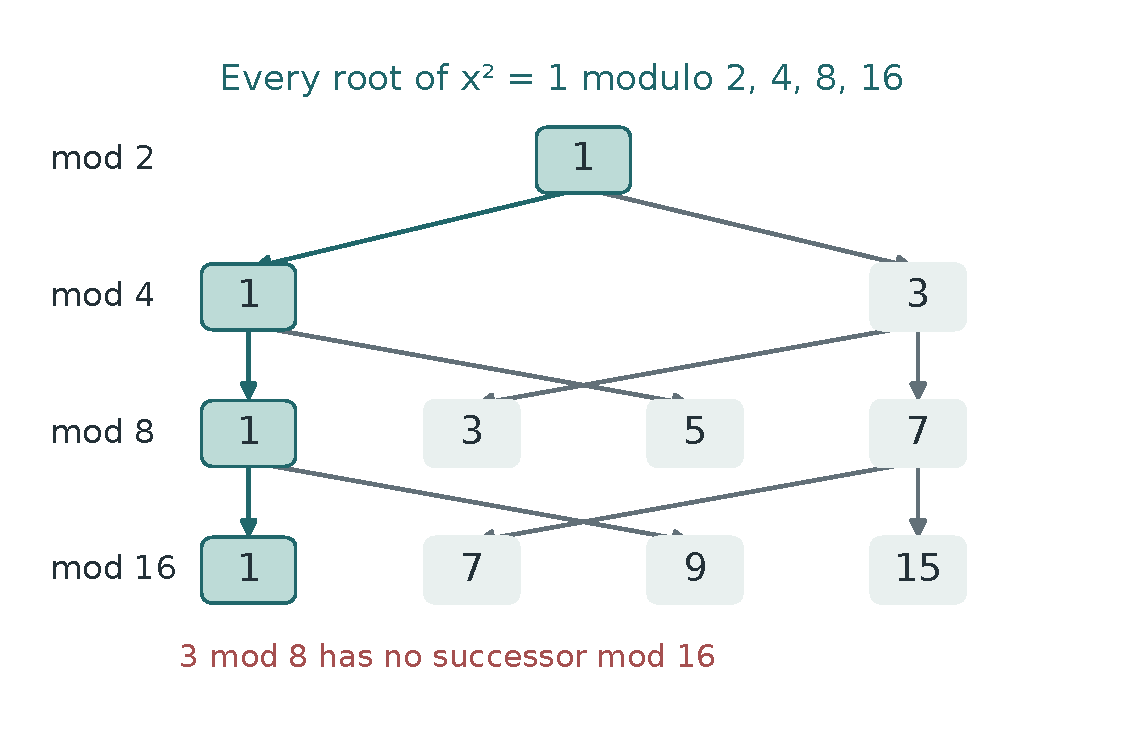
\includegraphics[width=.90\linewidth]{23_tower.pdf}
\caption{Scalar roots of one modulo successive powers of two form a finite prefix tree. A prefix can fail to continue even though other branches persist. An actual inverse limit needs a compatible branch at every depth. The separate matrix Hensel theorem supplies such a branch in its certified sector from one finite test.}
\label{fig:inverse_tower}\end{figure}
\section{Worked representation and selector calculations}\label{sec:worked_calculations}

The preceding arguments use a small number of mechanisms repeatedly. This section expands those mechanisms in examples that can be checked without automorphic input. The examples are finite representation models. An incompatible local model is not an arithmetic counterexample to Strong Artin.

\subsection{Why the prime cyclic Clifford alternative is exact}

\begin{proposition}[The two prime cyclic cases]\label{prop:worked_clifford}
Let \(G\) be finite, let \(H\triangleleft G\) with \(G/H\cong C_p\), and let \(V\) be irreducible over \(\CC\). Exactly one of the following occurs:
\begin{enumerate}
\item \(V|_H\) is irreducible and invariant under \(G\), and \(V\) is one of its \(p\) quotient character extensions.
\item \(V|_H\) is a sum of \(p\) pairwise nonisomorphic conjugate irreducible representations, and \(V\) is induced from any one of them.
\end{enumerate}
\end{proposition}

\begin{proof}
Complete reducibility for the finite subgroup gives an isotypic decomposition of \(V|_H\). The group \(G\) permutes these isotypic spaces by conjugating their types. More than one orbit would give a proper nonzero \(G\) stable direct sum, contrary to irreducibility. Thus there is one orbit. Since conjugation by \(H\) fixes isomorphism classes of \(H\) representations, the permutation action factors through \(C_p\). Its transitive orbit has size one or \(p\).

In the size \(p\) case, choose one isotypic space \(U\). Its translates are pairwise distinct isotypic spaces, with direct sum \(V\). The stabilizer of its type is exactly \(H\). If \(U\) had a proper nonzero \(H\) submodule, the direct sum of its \(p\) translates would be a proper nonzero \(G\) submodule of \(V\). Hence \(U\) is irreducible. The natural map from \(\Ind_H^G U\) to \(V\), sending each coset copy to its translated space, is an isomorphism. Its restriction is precisely the stated orbit sum.

In the size one case, write \(V|_H\cong\tau\otimes M\), where \(H\) acts trivially on the multiplicity space \(M\). The stable type \(\tau\) extends by \cref{lem:stable_extension}. Remove that extension action from the action on \(V\). The remaining action on \(M\) factors through \(C_p\). If \(M\) had a proper quotient stable subspace, its tensor product with \(\tau\) would give a proper \(G\) submodule of \(V\). Thus \(M\) is irreducible as a complex representation of \(C_p\). Every such irreducible is one dimensional. Therefore \(V|_H\cong\tau\), with multiplicity one, and the remaining quotient character is its extension label. The torsor theorem gives the \(p\) possible extensions. This proves both alternatives and excludes an intermediate multiplicity case.
\end{proof}

For a solvable finite group, a subnormal composition series has prime cyclic factors. Applied recursively to the constituents encountered along the series, this proposition separates induction steps from invariant extension steps. It does not say that every irreducible representation is induced all the way from a linear character. An invariant restriction can survive at positive rank. That surviving case is the attachment gate used in the main text.

For \(S_3\) and \(H=A_3\), the standard two dimensional representation lies in the moving case. A three cycle has the two nontrivial cube roots as eigenvalues. Restriction is the sum of the two nontrivial \(C_3\) characters. Induction from either one gives the standard representation. Its sign twist is isomorphic to itself. This self twist is allowed precisely because the restricted representation is reducible. It does not contradict freeness of the torsor whose restriction is irreducible.

\subsection{A rank three coefficient test that determinant misses}

Let \(\omega\) be a primitive cube root of unity and put
\[
 A=\operatorname{diag}(1,1,\omega).
\]
Expanding directly gives
\[
 \det(TI-A)
 =T^3-(2+\omega)T^2+(1+2\omega)T-\omega.
\]
The three elementary symmetric coefficients are
\[
 e_1=2+\omega,\qquad e_2=1+2\omega,\qquad e_3=\omega.
\]
For scalar twist \(\omega^jA\), they become
\[
 \omega^j(2+\omega),\qquad
 \omega^{2j}(1+2\omega),\qquad
 \omega^{3j}\omega=\omega.
\]
The determinant is constant for \(j=0,1,2\), but the first coefficient distinguishes the three labels because \(2+\omega\ne0\). Thus rank divisibility causes blindness of the determinant, rather than blindness of every coefficient.

Now compare the balanced matrix
\[
 A_{\mathrm{bal}}=\operatorname{diag}(1,\omega,\omega^2).
\]
Its polynomial is \(T^3-1\). Multiplying all eigenvalues by \(\omega\) merely permutes their multiset. Every lower coefficient vanishes, and the determinant is fixed. Its full characteristic polynomial is therefore blind to the label. This is an actual local rotational stabilizer. A claim that one characteristic polynomial always detects a quotient twist would fail on this example.

At quotient prime three and rank two, the determinant changes by \(\omega^{2j}\). If a required determinant ratio is \(\omega^b\), the unique candidate satisfies \(2j=b\) modulo three, so \(j=2b\). This solves a finite selection problem. It still does not show that every other coefficient of the candidate matches the target.

The all local comparison includes infinity. For a real place with complex quadratic extension, the quotient is \(C_2\). Let the target finite parameter have sign multiplicities \((3,0)\), and let a second parameter have multiplicities \((1,2)\). Both have determinant sign positive. Twisting the second by sign gives \((2,1)\), which still does not equal \((3,0)\). Its exact attachment set is empty. This is a finite local model showing why determinant selection, even with quotient prime coprime to rank, does not discharge the remaining infinity condition.

\subsection{Ordered multiplicities and a common shift}

Take \(G=C_2\times C_3\), let \(H=C_2\), and let \(\xi\) be the quotient character taking a generator of \(C_3\) to \(\omega\). Let \(\tau\) be the nontrivial character of \(H\), extended with trivial quotient action. Consider a semisimple representation with spectrum
\[
 P_{\tau,V}(z)=2+z.
\]
Its quotient multiplicity vector is \((2,1,0)\). Twisting by \(\xi\) gives
\[
 zP_{\tau,V}(z)=2z+z^2,
\]
whose vector is \((0,2,1)\). Twisting by \(\xi^2\) gives \((1,0,2)\). These are ordered vectors. Knowing that each has total multiplicity three does not retain the extension label.

Suppose a second stable \(H\) type \(\sigma\) occurs with spectrum one. If the target has spectra \(2z+z^2\) for \(\tau\) and \(z^2\) for \(\sigma\), the first block demands shift one and the second demands shift two. The two restrictions to \(H\) have the same multiplicities. Each block separately is a quotient twist of the matching source block. The full representation is not one quotient twist, because the required shifts disagree. This is the reason the spectrum criterion quantifies over one common \(j\), rather than an independent \(j_\tau\) for each type.

For a balanced multiplicity spectrum \(1+z+z^2\), both nonzero Fourier modes vanish:
\[
 1+\omega+\omega^2=0,\qquad
 1+\omega^2+\omega^4=0.
\]
The spectrum \(3\) has the same total multiplicity, but both nonzero modes equal three. Comparing only ratios for which the source mode is nonzero would omit both decisive comparisons. The zero support clause in \cref{def:local_spectral_obstruction} is therefore necessary. A zero source mode requires a zero target mode. It is not an instruction to skip that mode.

Changing the reference extension of \(\tau\) relabels both spectra by the same rotation. The attachment set does not change. Likewise changing the chosen generator of the quotient rescales all labels by an invertible element of \(\ZZ/p\ZZ\). These coordinate choices affect the displayed polynomials, but not the existence of an isomorphism after one common quotient twist.

For prime cyclic quotients a nonempty exact alignment set is either a singleton or all labels. Hence two nonempty exact singleton conditions \(\{1\}\) and \(\{2\}\) are incompatible, while \(\{1\}\) together with all labels is compatible. Coarse coefficient filters may produce other finite subsets, but those are not automatically exact extension spectrum sets. Keeping that distinction prevents a visual or computational filter from being assigned a stronger meaning than its construction supports.

\subsection{A trace encoding, with both hypothesis failures exposed}

Let
\[
 \Gamma=\{\operatorname{diag}(\omega^a,\omega^{-a}):a=0,1,2\}.
\]
The trace alphabet is \(\{2,-1\}\). The image algebra has dimension two, with basis the identity and \(\gamma_1=\operatorname{diag}(\omega,\omega^2)\). The trace coordinate map from \cref{thm:finite_trace_image_bound} gives
\[
 \Phi(\gamma_0)=(2,-1),\qquad
 \Phi(\gamma_1)=(-1,-1),\qquad
 \Phi(\gamma_2)=(-1,2).
\]
The tuples are distinct. The sharper algebra bound is \(3\le2^2=4\), while the rank only bound is \(3\le2^{2^2}=16\). The latter is deliberately rough. Its role is a uniform bound independent of the coefficient prime, not an efficient classification of the group.

Semisimplicity cannot be omitted. Over \(\CC\), the matrices
\[
 \begin{pmatrix}1&a\\0&1\end{pmatrix},\qquad a\in\ZZ,
\]
form an infinite group with the single trace value two. The invariant first coordinate line has no invariant complementary line. The trace pairing does not see the upper right nilpotent direction. This is exactly the step that fails without semisimplicity.

The characteristic restriction also has a visible purpose. In characteristic two, choose a primitive cube root \(\omega\) and the scalar group
\[
 \{I_2,\omega I_2,\omega^2 I_2\}.
\]
It is a faithful semisimple representation, as a direct sum of two identical one dimensional characters. Every trace is zero because its multiplicity two vanishes in the coefficient field. The alphabet has size one, but the group has size three. The would be bound \(3\le1^{4}\) is false. In the proof, the block pairing multiplier \(m_i=2\) is zero. Requiring \(\ell>n\) prevents precisely this multiplicity cancellation.

In characteristic zero the finite trace theorem itself is enough to prove finiteness once global semisimplicity and a finite image trace alphabet are known. The l adic part of the work is therefore not another mysterious finite image principle. It is the arithmetic passage from density one Frobenius data to the trace set of the full compact image, followed by this explicit algebraic encoding.

\subsection{A fixed alphabet and what a separating prime actually does}

For an elementary example, compare the integral polynomials
\[
 P(T)=T^2-2T+1,\qquad Q(T)=T^2+2T+1.
\]
Their middle coefficients differ by four. Reduction modulo two makes them equal. Reduction modulo any odd rational prime keeps them distinct. A separating prime is a coefficient prime with this latter injectivity property. It does not say which polynomial is realized by a global Galois representation. It says that, once a realization gives one of the alphabet polynomials modulo that prime, a different alphabet entry cannot imitate it.

For a cyclotomic alphabet over a number field, a nonzero algebraic integer difference has only finitely many prime ideal divisors. Choosing one nonzero coefficient difference for every pair therefore produces the finite bad set. Distinct roots can reduce to the same root at some bad prime, and repeated root multiplicities can become inseparable. The argument avoids those accidents by testing the polynomial alphabet, rather than presuming that each individual eigenvalue is already distinguished.

The large residual theorem uses two alphabets. One is the supplied automorphic alphabet. The other contains every degree \(n\) polynomial whose roots have orders at most \(B=t^{n^2}\). A field containing \(\mu_{\operatorname{lcm}(1,\ldots,B)}\) contains all their coefficients. Both the field and the exceptional coefficient primes are fixed before choosing a residual realization. This order matters. A proof that chose a separation field from the coefficients of an as yet unknown lift and then called the excluded primes a predetermined set would leave a circular quantifier.

The resulting bound is not claimed to be practical. Even \(t\) and \(n\) of moderate size make \(B\) and the universal cyclotomic field enormous. The theorem establishes an existence implication with a finite exceptional set. A useful computational implementation for a particular finite image may exploit its actual exponent and much smaller image algebra, but that is an additional optimization and must retain the same separation logic.

\section{Statement map and the remaining arithmetic obligation}\label{sec:statement_map}

The reader edition has three layers of evidence. The finite algebra proofs in the main text and local appendix are written out. Classical automorphic, local Langlands, and representation realization results are imported with their source hypotheses. The formal archive records exactly encoded algebraic theorems and historical build evidence. These layers support one another without being interchangeable.

\begin{longtable}{>{\raggedright\arraybackslash}p{.24\linewidth}>{\raggedright\arraybackslash}p{.33\linewidth}>{\raggedright\arraybackslash}p{.34\linewidth}}
\toprule
Statement group & What the proof supplies & What remains an input\\
\midrule
\endfirsthead
\toprule
Statement group & What the proof supplies & What remains an input\\
\midrule
\endhead
Cyclic extension torsor & All extensions of one invariant irreducible type differ by a unique quotient character & An automorphic attachment to select the matching extension\\
Coefficient and multiplicity selectors & Exact rotation, stabilizer, and common shift tests & Actual local data and compatibility of the selected global label\\
Finite Satake descent & A bounded root of unity alphabet outside a finite exceptional set & The known lower automorphic correspondence and base change compatibility\\
Trace encoding & Finite image and the bound under semisimplicity and characteristic hypotheses & A representation whose trace alphabet has the required form\\
Separating residual recovery & Exact weak characteristic zero attachment from a supplied good residual realization & Existence of that residual realization and remaining local checks\\
Large residual recovery & A finite ordinary lift and exact alphabet recovery at sufficiently large good primes & The residual representation and classical cross characteristic lifting theorem\\
Quotient prime congruence & Equal reduced unramified polynomial systems with collapsed labels & A suitable weight zero lifting theorem with target local control\\
Semisimple l adic rigidity & Finite image from continuous finitely ramified realization and finite Frobenius traces & Existence and exact polynomial normalization of that realization\\
Cyclic cohomology and syzygies & Algebraic spaces, redundancy relations, and conditional local obstruction criteria & Arithmetic Selmer comparison and the required terminal obstruction vanishing\\
Certified matrix Hensel sector & Unique actual local root from one finite test when \(m>s\) and the two sided inverse certificate holds & A certificate, singular sector analysis, and arithmetic or global realization\\
Solvable recursion & A complete implication from gates at every invariant step & Uniformly supplying those gates over the encountered fields and ranks\\
\bottomrule
\end{longtable}

The historical paper contains additional theorem statements, corollaries, and small example verifiers. Its source and audit are retained as evidence, with the current statement map recording the narrowed claims used in this edition. The older global semisimplicity, Fourier zero support, coefficient field, and exceptional place issues have been corrected in the reader text. The later formal checkpoints are not retroactive certificates of every classical theorem or every prose argument in that historical paper.

The remaining global question can now be stated without a vague final step. At an invariant cyclic restriction, the automorphic descent fibre is known to exist. Can one prove that a descent has a continuous Galois realization with the exact normalized polynomial data, or lift the canonical quotient prime congruence to the prescribed target with its local conditions? If the answer supplies only almost everywhere polynomials, the exceptional finite and archimedean conditions must still be addressed for the all local version.

This is an existence and compatibility obligation. A finite trace alphabet controls a representation after it exists. A syzygy certificate removes redundant equations after the deformation comparison is supplied. A Hensel certificate solves a specified local matrix equation in its certified ball. None of those conclusions creates the global automorphic to Galois arrow by itself. Their value is that the resulting arrow, when constructed, will arrive at a tightly constrained and independently checkable destination.

\begingroup\small\raggedright
\begin{thebibliography}{99}
\bibitem{ArthurClozel1989}
J. Arthur and L. Clozel, \emph{Simple Algebras, Base Change, and the Advanced Theory of the Trace Formula}, Annals of Mathematics Studies 120, Princeton University Press, 1989. Prime cyclic base change and induction are used with their cuspidality hypotheses.

\bibitem{ClozelRajan2020}
L. Clozel and C. S. Rajan, Solvable base change, \emph{Journal f\"ur die reine und angewandte Mathematik} 772 (2021), 147--174. DOI: \href{https://doi.org/10.1515/crelle-2020-0023}{10.1515/crelle-2020-0023}. Checked preprint \href{https://arxiv.org/abs/1806.02513}{arXiv:1806.02513v1}, 7 June 2018. Theorem 3(2) and the ensuing cyclic descent remark are the fibre inputs.

\bibitem{Rajan2002}
C. S. Rajan, On the image and fibres of solvable base change, \emph{Mathematical Research Letters} 9 (2002), 499--508.

\bibitem{KimYamauchi2016}
H. H. Kim and T. Yamauchi, A uniform structure on subgroups of \(GL_n(\mathbb F_q)\) and its application to a conditional construction of Artin representations of \(GL_n\), \emph{Journal of the Ramanujan Mathematical Society} 32(1) (2017), 75--99. Checked preprint \href{https://arxiv.org/abs/1403.5535}{arXiv:1403.5535v3}, 7 April 2016. Theorem 1.1 is conditional on its five inputs. The inherited citation key records the preprint year.

\bibitem{Ramakrishnan2002}
D. Ramakrishnan, Modularity of solvable Artin representations of \(GO(4)\) type, \emph{International Mathematics Research Notices} 2002(1), 1--54. DOI: \href{https://doi.org/10.1155/S1073792802000016}{10.1155/S1073792802000016}.

\bibitem{Langlands1980}
R. P. Langlands, \emph{Base Change for \(GL(2)\)}, Annals of Mathematics Studies 96, Princeton University Press, 1980.

\bibitem{Tunnell1981}
J. Tunnell, Artin's conjecture for representations of octahedral type, \emph{Bulletin of the American Mathematical Society} 5(2) (1981), 173--175.

\bibitem{Neukirch1999}
J. Neukirch, \emph{Algebraic Number Theory}, Springer, 1999.

\bibitem{Henniart2000}
G. Henniart, Une preuve simple des conjectures de Langlands pour \(GL(n)\) sur un corps p-adique, \emph{Inventiones Mathematicae} 139(2) (2000), 439--455.

\bibitem{HarrisTaylor2001}
M. Harris and R. Taylor, \emph{The Geometry and Cohomology of Some Simple Shimura Varieties}, Annals of Mathematics Studies 151, Princeton University Press, 2001. Checked author preprint dated 30 August 1999, Lemma 12.7(4--6), for twisting, cyclic prime base change, and induction compatibility. Its numbering differs from the published book.

\bibitem{Brauer1947}
R. Brauer, On Artin's \(L\)-series with general group characters, \emph{Annals of Mathematics} 48 (1947), 502--514.

\bibitem{Konig2010}
J. K\"onig, Solvability of generalized monomial groups, \emph{Journal of Group Theory} 13(2) (2010).

\bibitem{CimpoeasNicolae2020}
M. Cimpoea\c{s} and F. Nicolae, Artin \(L\)-functions of almost monomial Galois groups, \emph{Forum Mathematicum} 32(4) (2020).

\bibitem{Brown1982}
K. S. Brown, \emph{Cohomology of Groups}, Graduate Texts in Mathematics 87, Springer, 1982.

\bibitem{Isaacs1976}
I. M. Isaacs, \emph{Character Theory of Finite Groups}, Academic Press, 1976.

\bibitem{Chenevier2014}
G. Chenevier, The p-adic analytic space of pseudocharacters of a profinite group and pseudorepresentations over arbitrary rings, in \emph{Automorphic Forms and Galois Representations}, Vol. 1, London Mathematical Society Lecture Note Series 414, Cambridge University Press, 2014, 221--285. DOI: \href{https://doi.org/10.1017/CBO9781107446335.008}{10.1017/CBO9781107446335.008}. Checked \href{https://arxiv.org/abs/0809.0415}{arXiv:0809.0415v2}, 18 July 2013: Proposition 1.27, Theorem 2.12, Corollary 2.13, and Section 4.1. These are preprint numbering. The algebraic realization theorem alone does not assert continuity for the usual complex or l-adic topology.

\bibitem{Scholze2015}
P. Scholze, On torsion in the cohomology of locally symmetric varieties, \emph{Annals of Mathematics} 182(3) (2015), 945--1066. DOI: \href{https://doi.org/10.4007/annals.2015.182.3.3}{10.4007/annals.2015.182.3.3}. Corollary 5.4.3, p. 1060, is the residual eigensystem input. Field conditions, cohomological occurrence, normalization, and the source's historical dependencies are retained.

\bibitem{GoldringShin2014}
W. Goldring, with an appendix by S. W. Shin, Galois representations associated to holomorphic limits of discrete series, \emph{Compositio Mathematica} 150(2) (2014), 191--228. DOI: \href{https://doi.org/10.1112/S0010437X13007355}{10.1112/S0010437X13007355}. Theorem 1.2.1 is used only with its unitary datum, coefficient prime, and split prime normalization conditions.

\bibitem{GeeKassaei2013}
T. Gee and P. Kassaei, Companion forms in parallel weight one, \emph{Compositio Mathematica} 149(6) (2013), 903--913. DOI: \href{https://doi.org/10.1112/S0010437X12000875}{10.1112/S0010437X12000875}. Checked \href{https://arxiv.org/abs/1206.6631}{arXiv:1206.6631v1}, 28 June 2012. Its companion and Artin consequences retain their respective modularity hypotheses.

\bibitem{DimitrovWiese2020}
M. Dimitrov and G. Wiese, Unramifiedness of Galois representations attached to Hilbert modular forms mod \(p\) of weight one, \emph{Journal of the Institute of Mathematics of Jussieu} 19(2) (2020), 281--306. DOI: \href{https://doi.org/10.1017/S1474748018000026}{10.1017/S1474748018000026}. Checked preprint version 4, 28 November 2017. The full Frobenius polynomial comparison also requires the diamond character determinant normalization.

\bibitem{BrauerNesbitt1941}
R. Brauer and C. Nesbitt, On the modular characters of groups, \emph{Annals of Mathematics} 42(2) (1941), 556--590.

\bibitem{CurtisReiner1962}
C. W. Curtis and I. Reiner, \emph{Representation Theory of Finite Groups and Associative Algebras}, John Wiley and Sons, 1962.

\bibitem{Serre1977}
J.-P. Serre, \emph{Linear Representations of Finite Groups}, Graduate Texts in Mathematics 42, Springer, 1977.

\bibitem{Deligne1973}
P. Deligne, Les constantes des \'equations fonctionnelles des fonctions \(L\), in \emph{Modular Functions of One Variable II}, Lecture Notes in Mathematics 349, Springer, 1973, 501--597.

\bibitem{DeligneHenniart1981}
P. Deligne and G. Henniart, Sur la variation, par torsion, des constantes locales d'\'equations fonctionnelles de fonctions \(L\), \emph{Inventiones Mathematicae} 64(1) (1981), 89--118. Theorem 4.6, p. 110, supplies the stable epsilon ratio used here.

\bibitem{BLGGT2014}
T. Barnet-Lamb, T. Gee, D. Geraghty, and R. Taylor, Potential automorphy and change of weight, \emph{Annals of Mathematics} 179(2) (2014), 501--609. DOI: \href{https://doi.org/10.4007/annals.2014.179.2.3}{10.4007/annals.2014.179.2.3}. Checked \href{https://arxiv.org/abs/1010.2561}{arXiv:1010.2561v4}, 9 December 2013. Theorem 4.2.1 uses regular algebraic and further lifting hypotheses.

\bibitem{CalegariGeraghty2020}
F. Calegari and D. Geraghty, Minimal modularity lifting for nonregular symplectic representations, \emph{Duke Mathematical Journal} 169(5) (2020), 801--896. DOI: \href{https://doi.org/10.1215/00127094-2019-0044}{10.1215/00127094-2019-0044}. This is a special nonregular range, not the arbitrary all zero weight gate.

\bibitem{DeligneSerre1974}
P. Deligne and J.-P. Serre, Formes modulaires de poids 1, \emph{Annales scientifiques de l'\'Ecole Normale Sup\'erieure} 7(4) (1974), 507--530. DOI: \href{https://doi.org/10.24033/asens.1277}{10.24033/asens.1277}. Lemma 3.2, p. 513, is a primary instance of the Frobenius determination argument.

\bibitem{Wang2026}
J. Wang, Strong Artin conjecture for generalized octahedral representations in \(GL_3\), \href{https://arxiv.org/abs/2609.38231}{arXiv:2609.38231v1}, 28 September 2026. Theorem 1.1 and Corollary 5.4 state the special three and six dimensional cases mentioned here. Statements checked. The full proof has not been independently audited for this reader edition.
\end{thebibliography}

\endgroup
\end{document}
